\chapter{LFV analysis background estimation}

\subsection{Background estimates for $\Hmuhad$}


\subsubsection{Misidentified Leptons}

The misidentified lepton backgrounds are estimated with full data driven method from the collision data. In $\Hmuhad$ channel, the misidentification $\tau$ and $\mu$ lepton rate is obtained from independent Z + jets data sets and then apply the rate to a control region that orthogonal to the signal region to estimate the misidentified lepton backgrounds.  The control regions for the estimation and validation of the misidentified lepton background are shown in Table.~\ref{tab:fakeratediagram}. Region I is the signal region with full selection applied. Region III is the background enriched region, in which one or two leptons have loose isolation but not tight isolation. Region II is the same to Region I besides the requirement that $\mu$ and $\tau$ lepton pairs have the same sign of charge, so as Region IV to Region III. Region III is used to estimate the misidentified background in Region I. Region II and IV are used in the validation of the method. 


\begin{table}[hbt]
 \centering
 {
 \renewcommand{\arraystretch}{1.1}
 \caption{Definition of the samples used to estimate the misidentified lepton background.}
  \label{tab:fakeratediagram}
  \begin{tabular}{c|c} \hline
\textbf{Region I}              &  \textbf{Region II}             \\ \hline
$\ell^{\pm}_{1}$(isolated)  &  $\ell^{\pm}_{1}$(isolated)             \\
$\ell^{\mp}_{2}$(isolated)  &  $\ell^{\pm}_{2}$(isolated)             \\

\hline \hline
\textbf{Region III}           &  \textbf{Region IV}             \\ \hline
$\ell^{\pm}_{1}$(isolated)  &  $\ell^{\pm}_{1}$(isolated)             \\
$\ell^{\mp}_{2}$(not-isolated )  &  $\ell^{\pm}_{2}$(not-isolated)             \\
\hline
  \end{tabular}
}
\end{table}



$Z\rightarrow\mu\mu$ is used in Z + jets data sets to estimate both misidentified $\tau$ and $\mu$ lepton rates. Z bosons are selected in the invariant mass window $70<M_{ll}<110$ GeV and trigger HLT\_IsoMu24 or HLT\_IsoTkMu24 is used in the selection. Two muons that are composed of Z bosons are required to have $\pt>26$ GeV, $|\eta|<2.4$, cut based tight muon isolation($I^{\mu}_{rel}<0.15$) and passing the muon medium ID. In the Z+jets samples, with the selected Z boson in an event, the remaining jets are checked if they pass $\tau$ or $\mu$ selection.

To estimate the misidentified $\tau$ lepton rate, The jets in the sample Z + jets are checked if they pass the $\tau$ isolation ID. Misidentified $\tau$ lepton ratio $\tau(f_{\tau})$ is calculated as in Equation .~\ref{eq:fakerate1}, together with one related ratio $f_{\tau}$. In Equation .~\ref{eq:fakerate1}, $\ell$ stands for leptons in general.

\begin{align} 
\ell(f_{\ell})&=\frac{f_{\ell}}{1-f_{\ell}} \label{eq:fakerate1}\\
f_{\ell}&=\frac{N_{\ell}(Z+jets\ \ell \ tight\ Iso)}{N_{\tau}(Z+jets\ \ell \ loose\ Iso)} \label{eq:fakerate2}
\end{align}

$f_{\tau}$ is the ratio between number of jets that pass tight $\tau$ MVA isolation ID and number of jets that pass very loose $\tau$ MVA isolation ID. The contribution from Diboson sample is subtracted with simulation, in which the third leptons are genuine leptons. With the ratio $f_{\tau}$ , misidentified rate $\tau(f_{\tau})$(Equation.~\ref{eq:fakerate2}) is applied as a weight to Region III. When estimating misidentified $tau$ leptons, Region III is defined in the same selection condition as the signal region Region I , but  $\tau$ leptons are required to pass the very loose MVA isolation and not pass the tight MVA isolation. The misidentified $\tau$ lepton rate $\tau(f_{\tau})$ shows dependence on tau $\pt$, tau decay mode and ECAL geometry. Thus $\tau(f_{\tau})$ is applied in term of tau $\pt$, tau decay modes and ECAL barrel and endcap seperately. The distribution of $f_{\tau}$ is shown in Fig.~ \ref{fig:fakerationumber}, which shows a comparison of the estimated $f_{\tau}$ between data and simulated Z+jets samples. The distribution of $f_{\tau}$ vs $|\eta|$ are also shown, which show less dependency. 

\begin{figure}[htbp] 
     \centering
     \subfigure[EB tau decay mode 0]{ 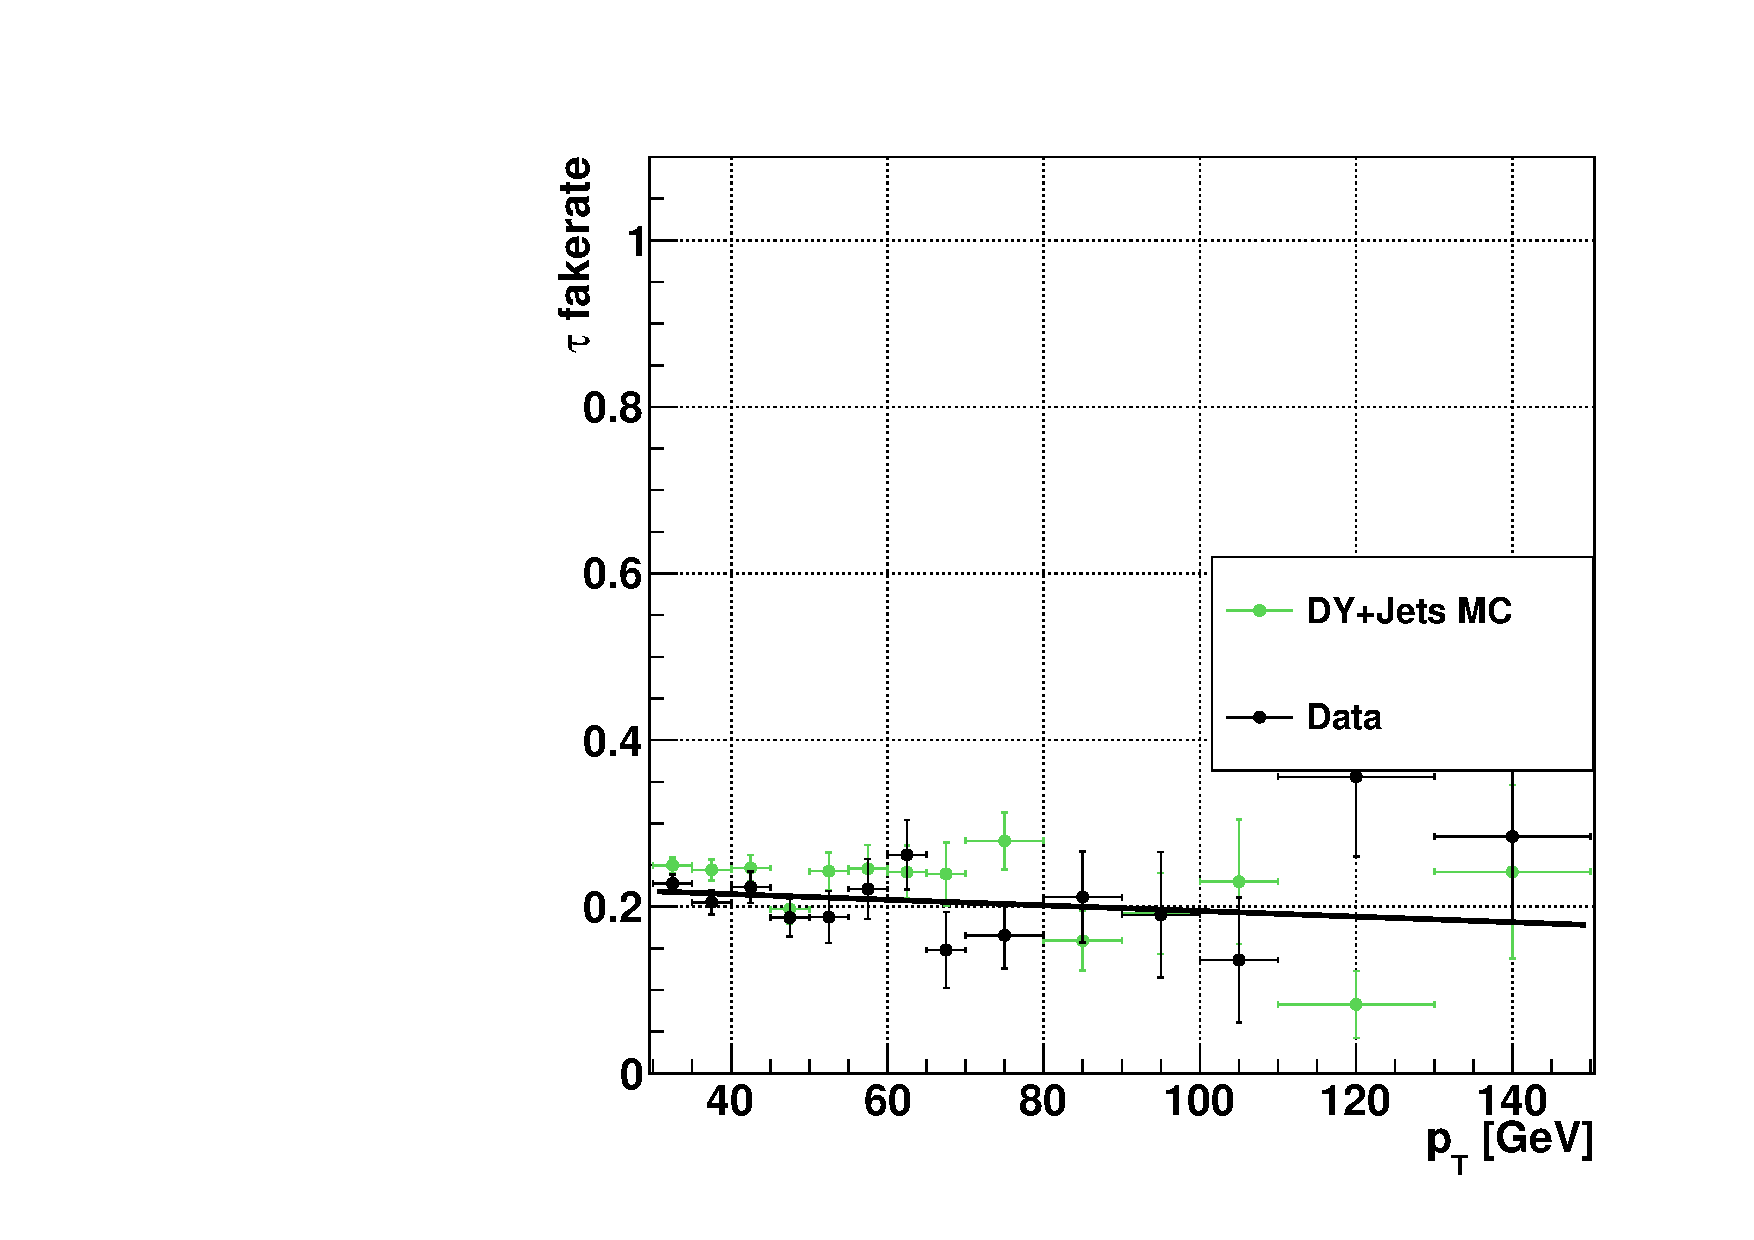
\includegraphics[width=0.3\textwidth]{chapter6/t_DM0EB_tPt_fakeRate.pdf}}
      \subfigure[EB tau decay mode 1]{ 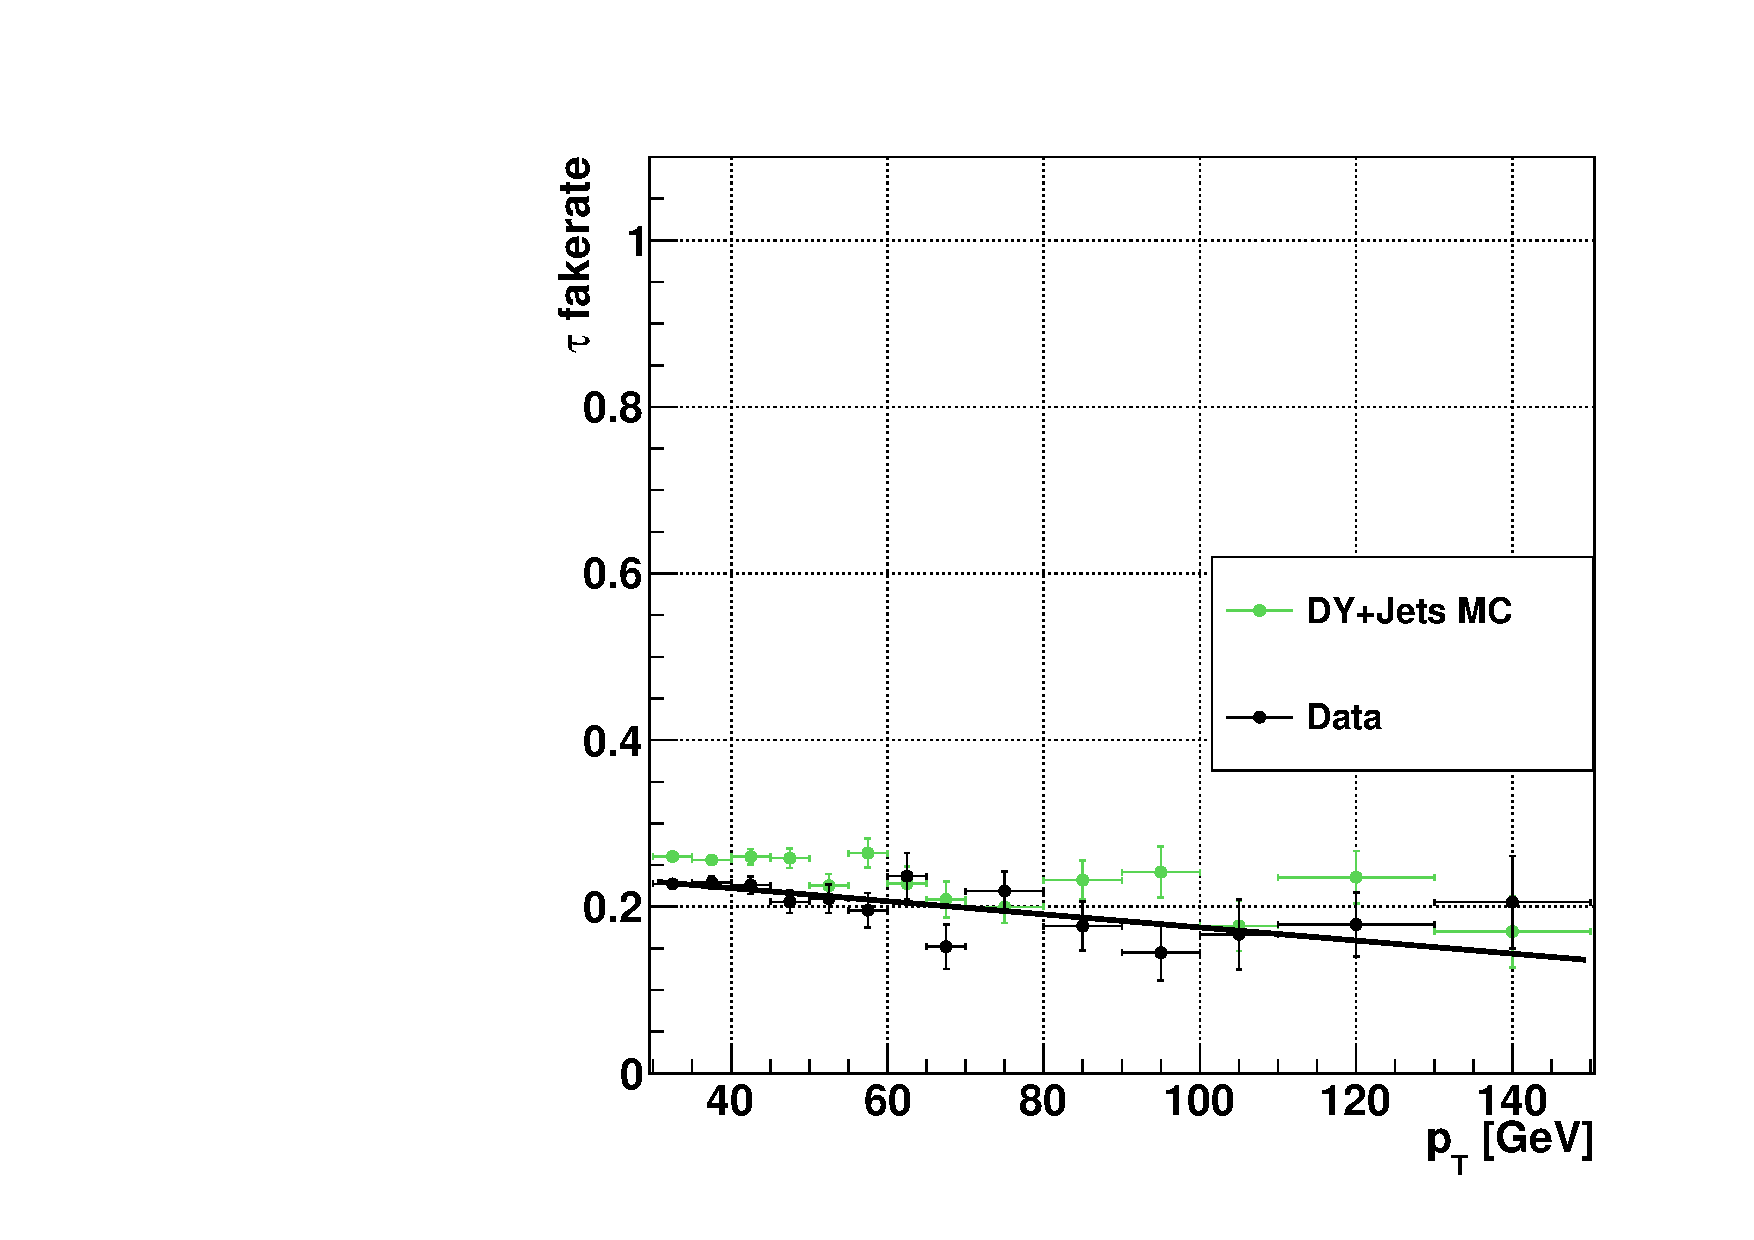
\includegraphics[width=0.3\textwidth]{chapter6/t_DM1EB_tPt_fakeRate.pdf}}
      \subfigure[EB tau decay mode 10]{ 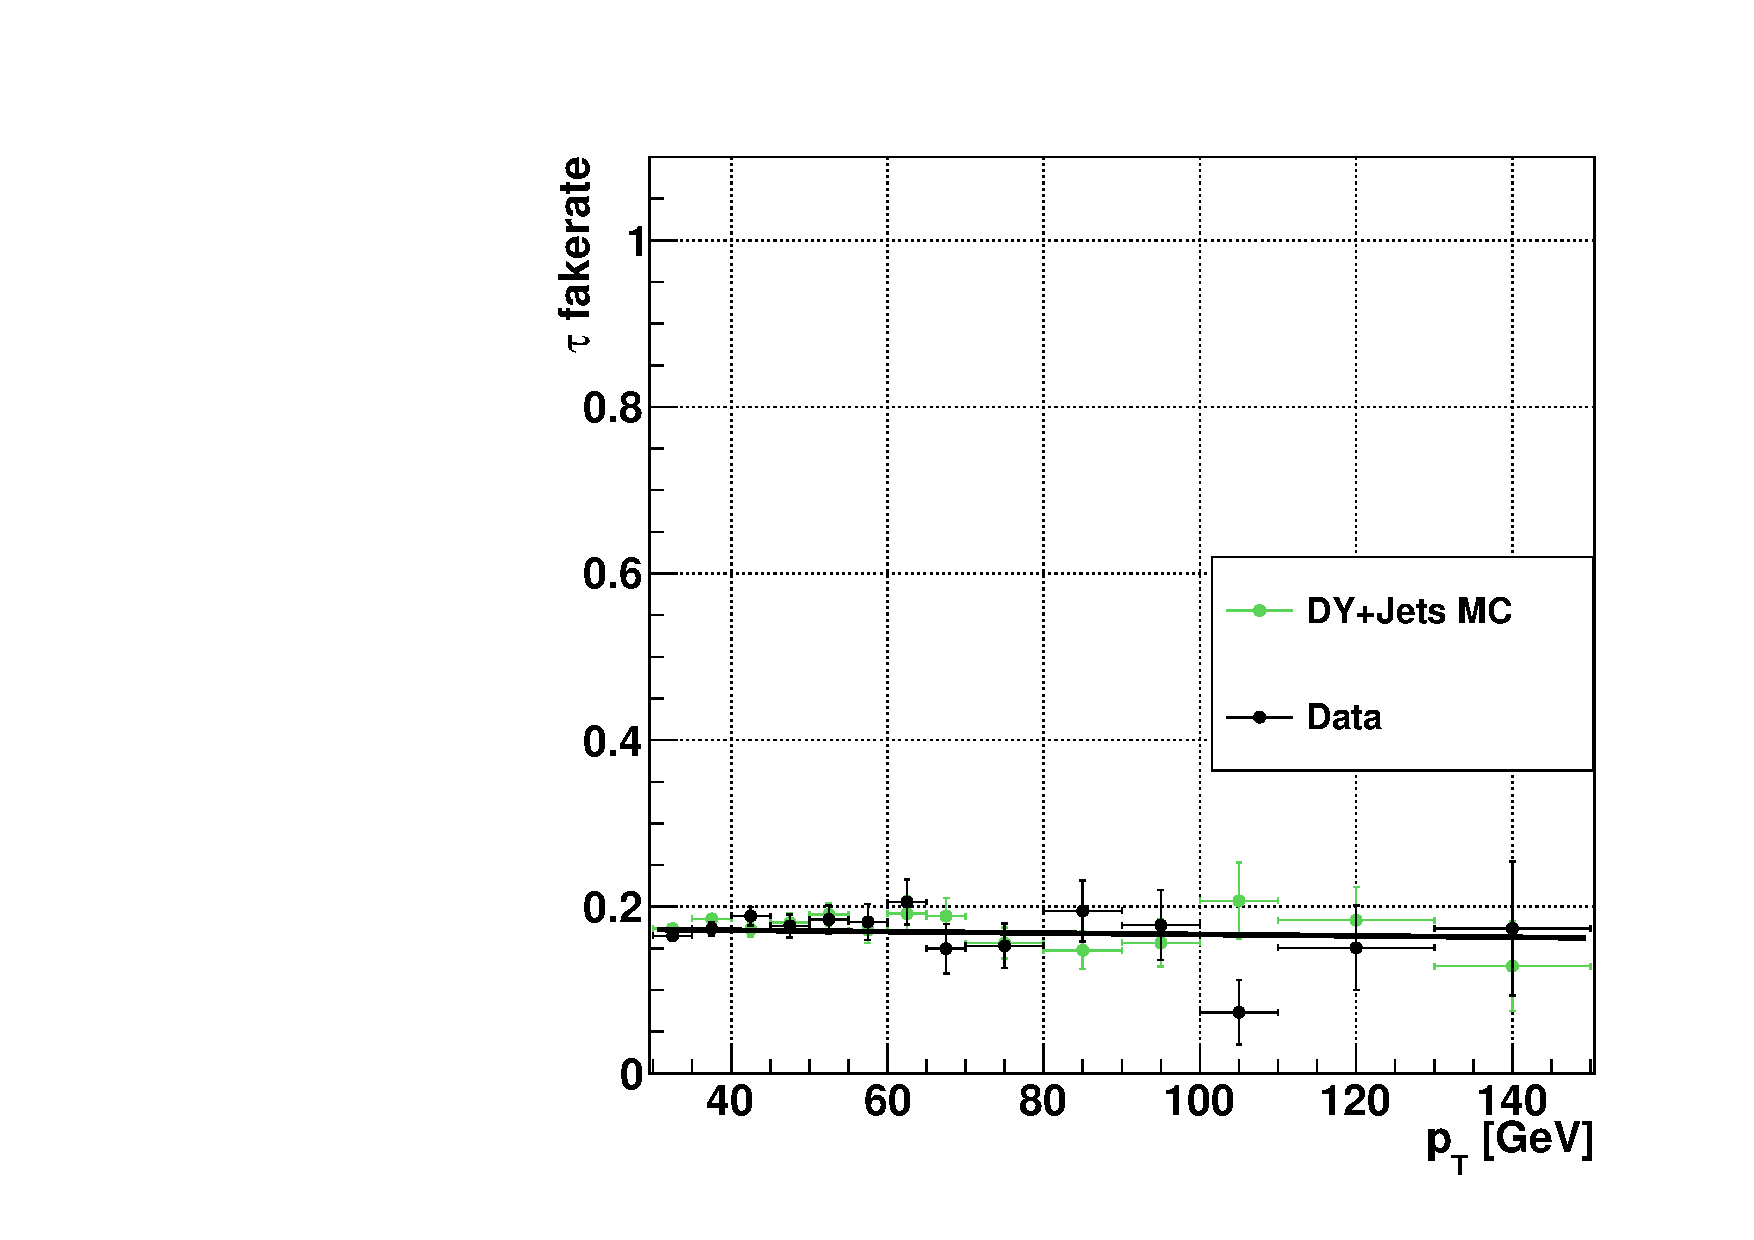
\includegraphics[width=0.3\textwidth]{chapter6/t_DM10EB_tPt_fakeRate.pdf}}
     \subfigure[EE tau decay mode 0]{ 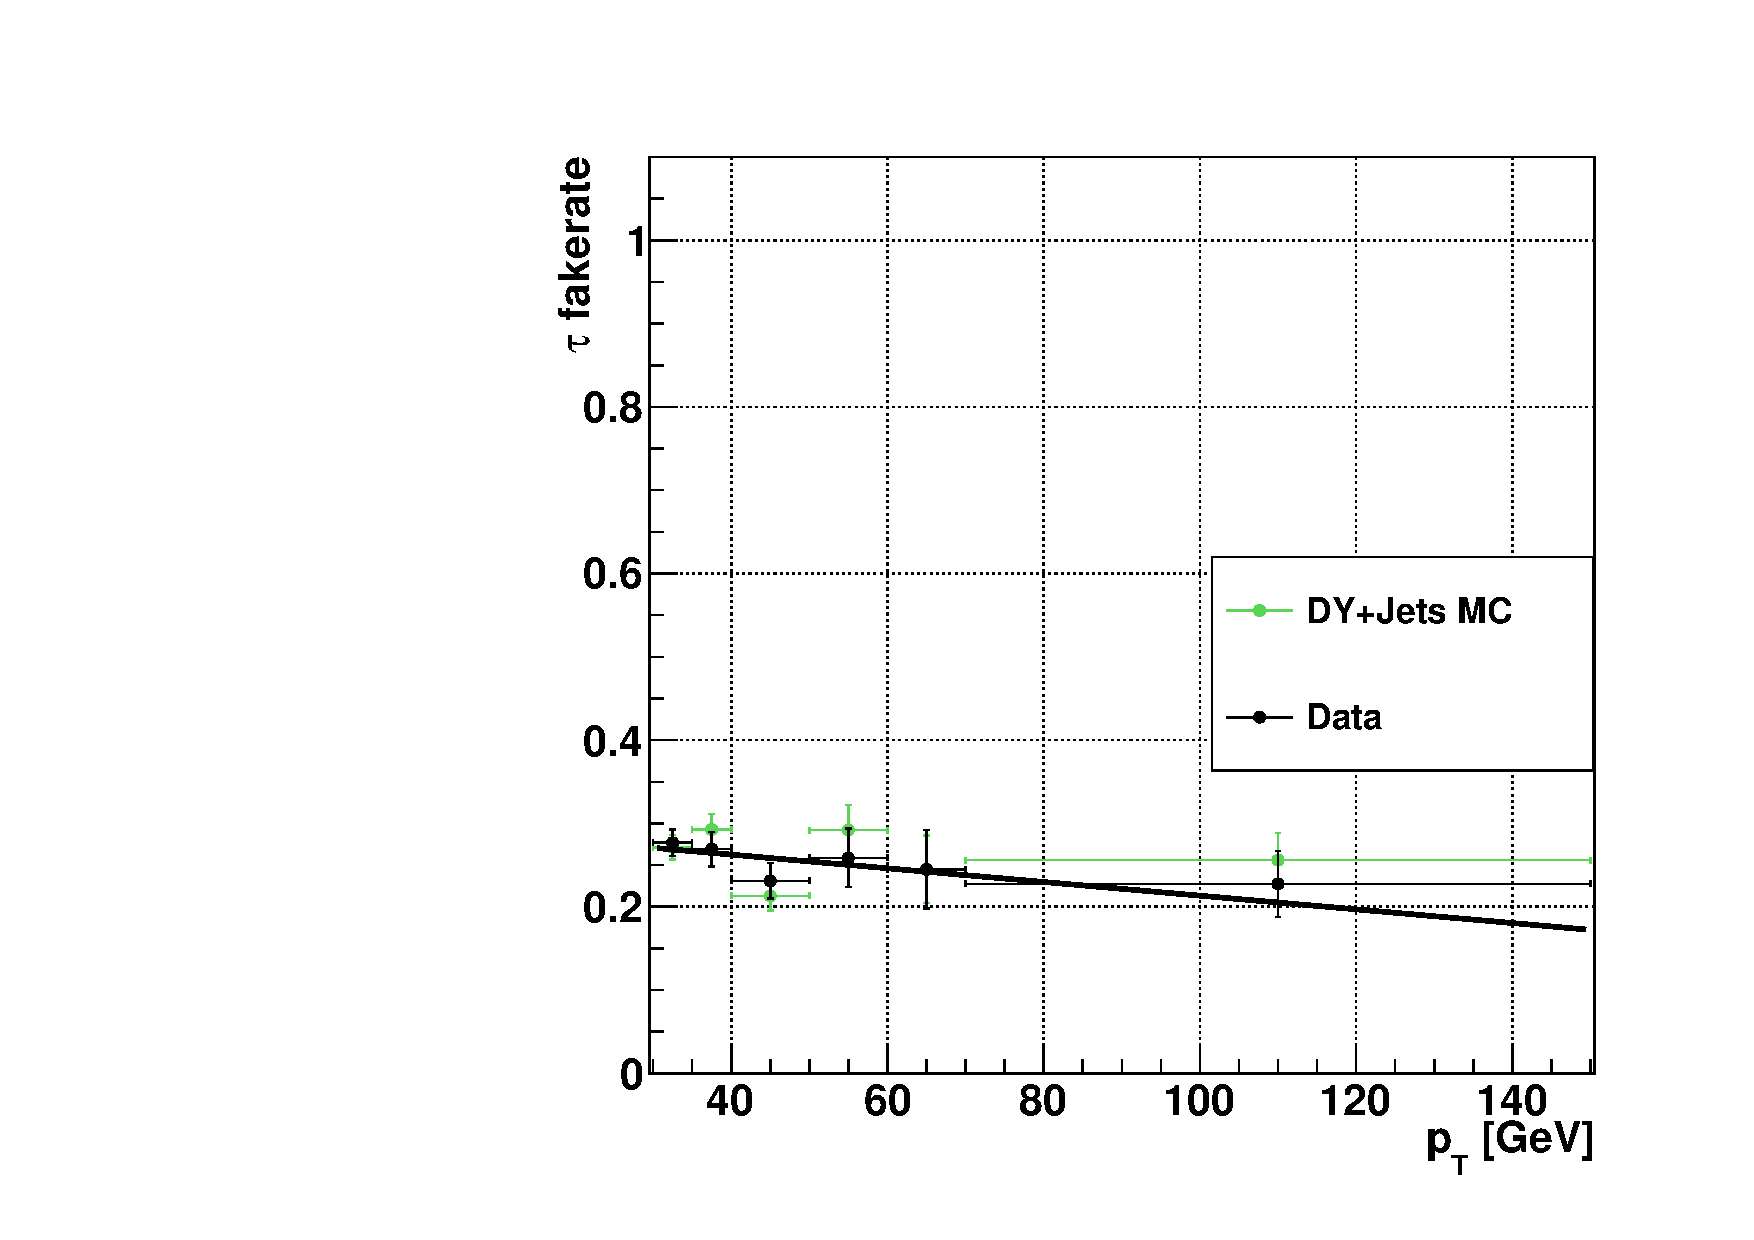
\includegraphics[width=0.3\textwidth]{chapter6/t_DM0EE_tPt_fakeRate.pdf}}
      \subfigure[EE tau decay mode 1]{ 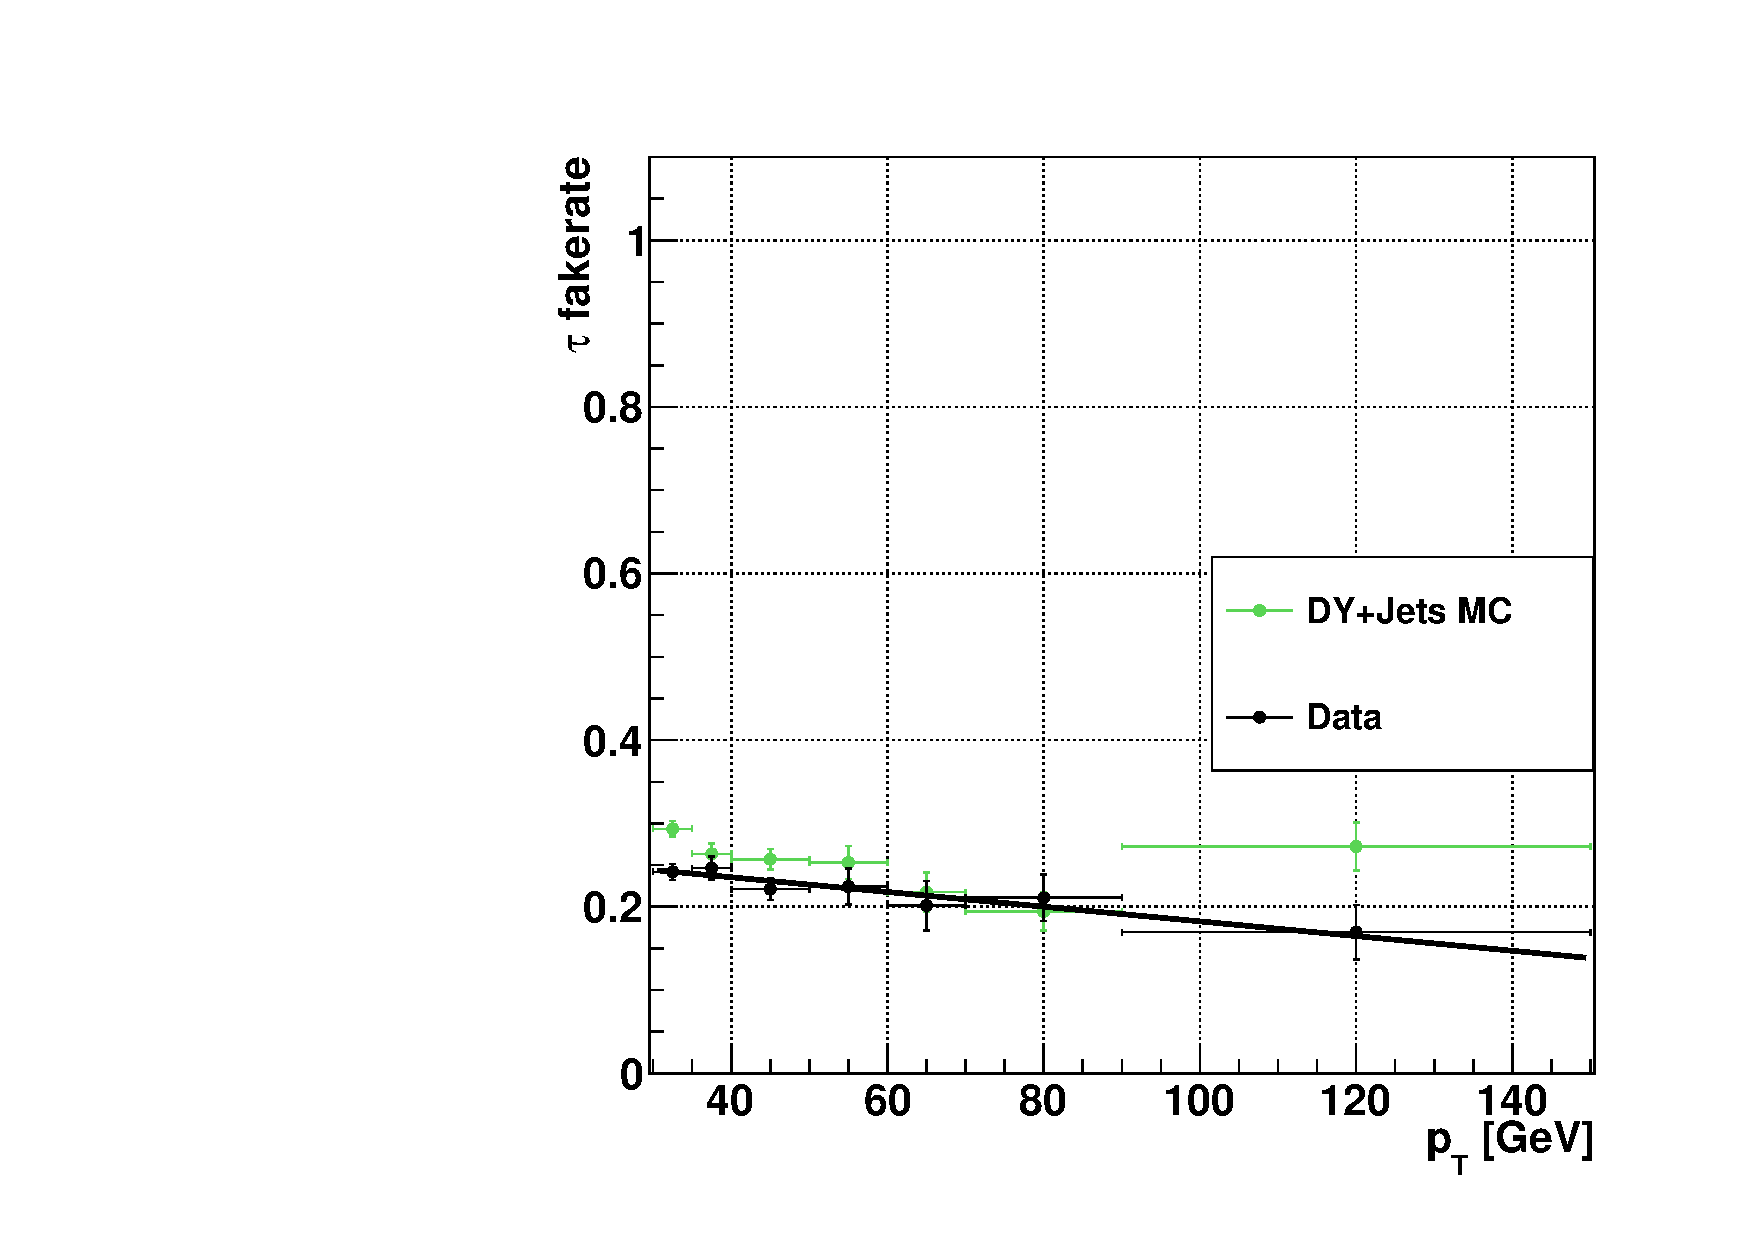
\includegraphics[width=0.3\textwidth]{chapter6/t_DM1EE_tPt_fakeRate.pdf}}
      \subfigure[EE tau decay mode 10]{ 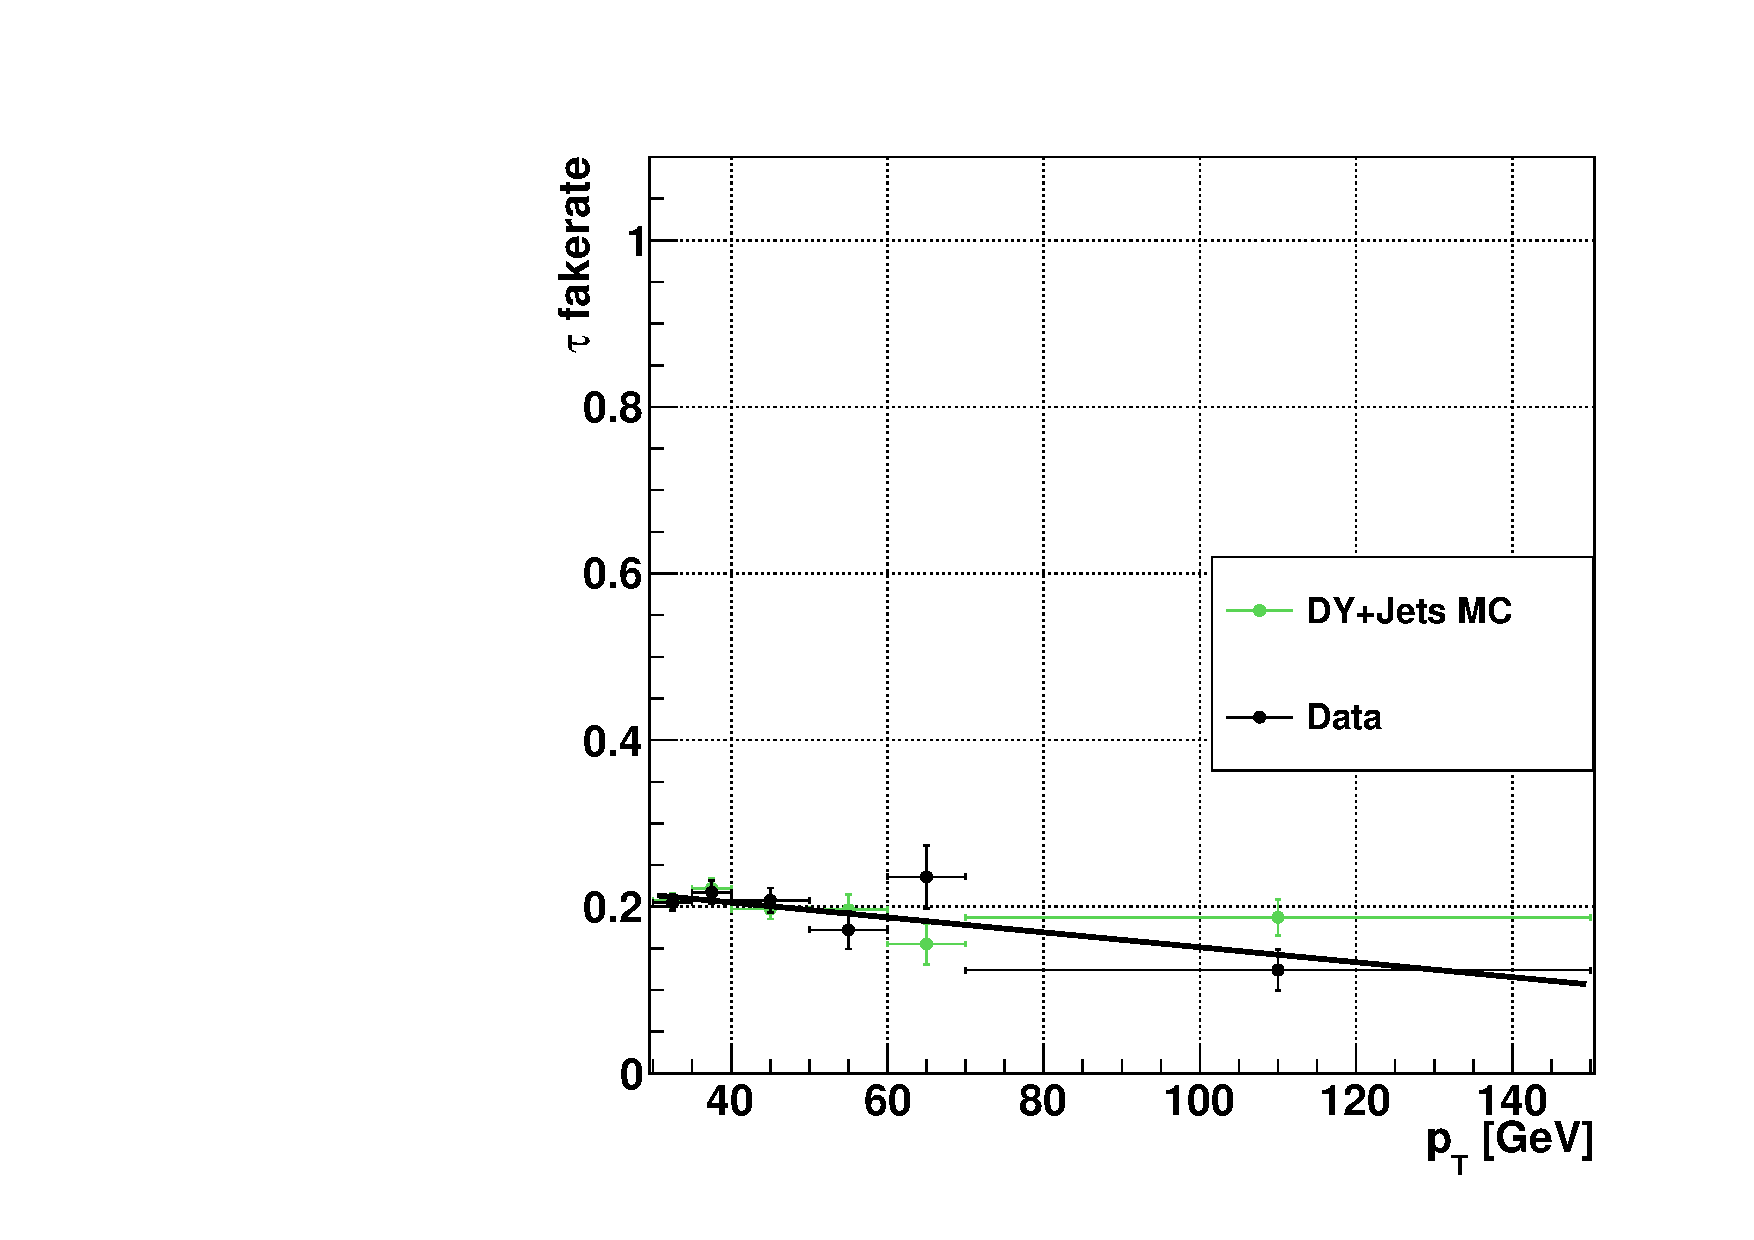
\includegraphics[width=0.3\textwidth]{chapter6/t_DM10EE_tPt_fakeRate.pdf}}
       \subfigure[tau decay mode 0 vs $|\eta|$]{ 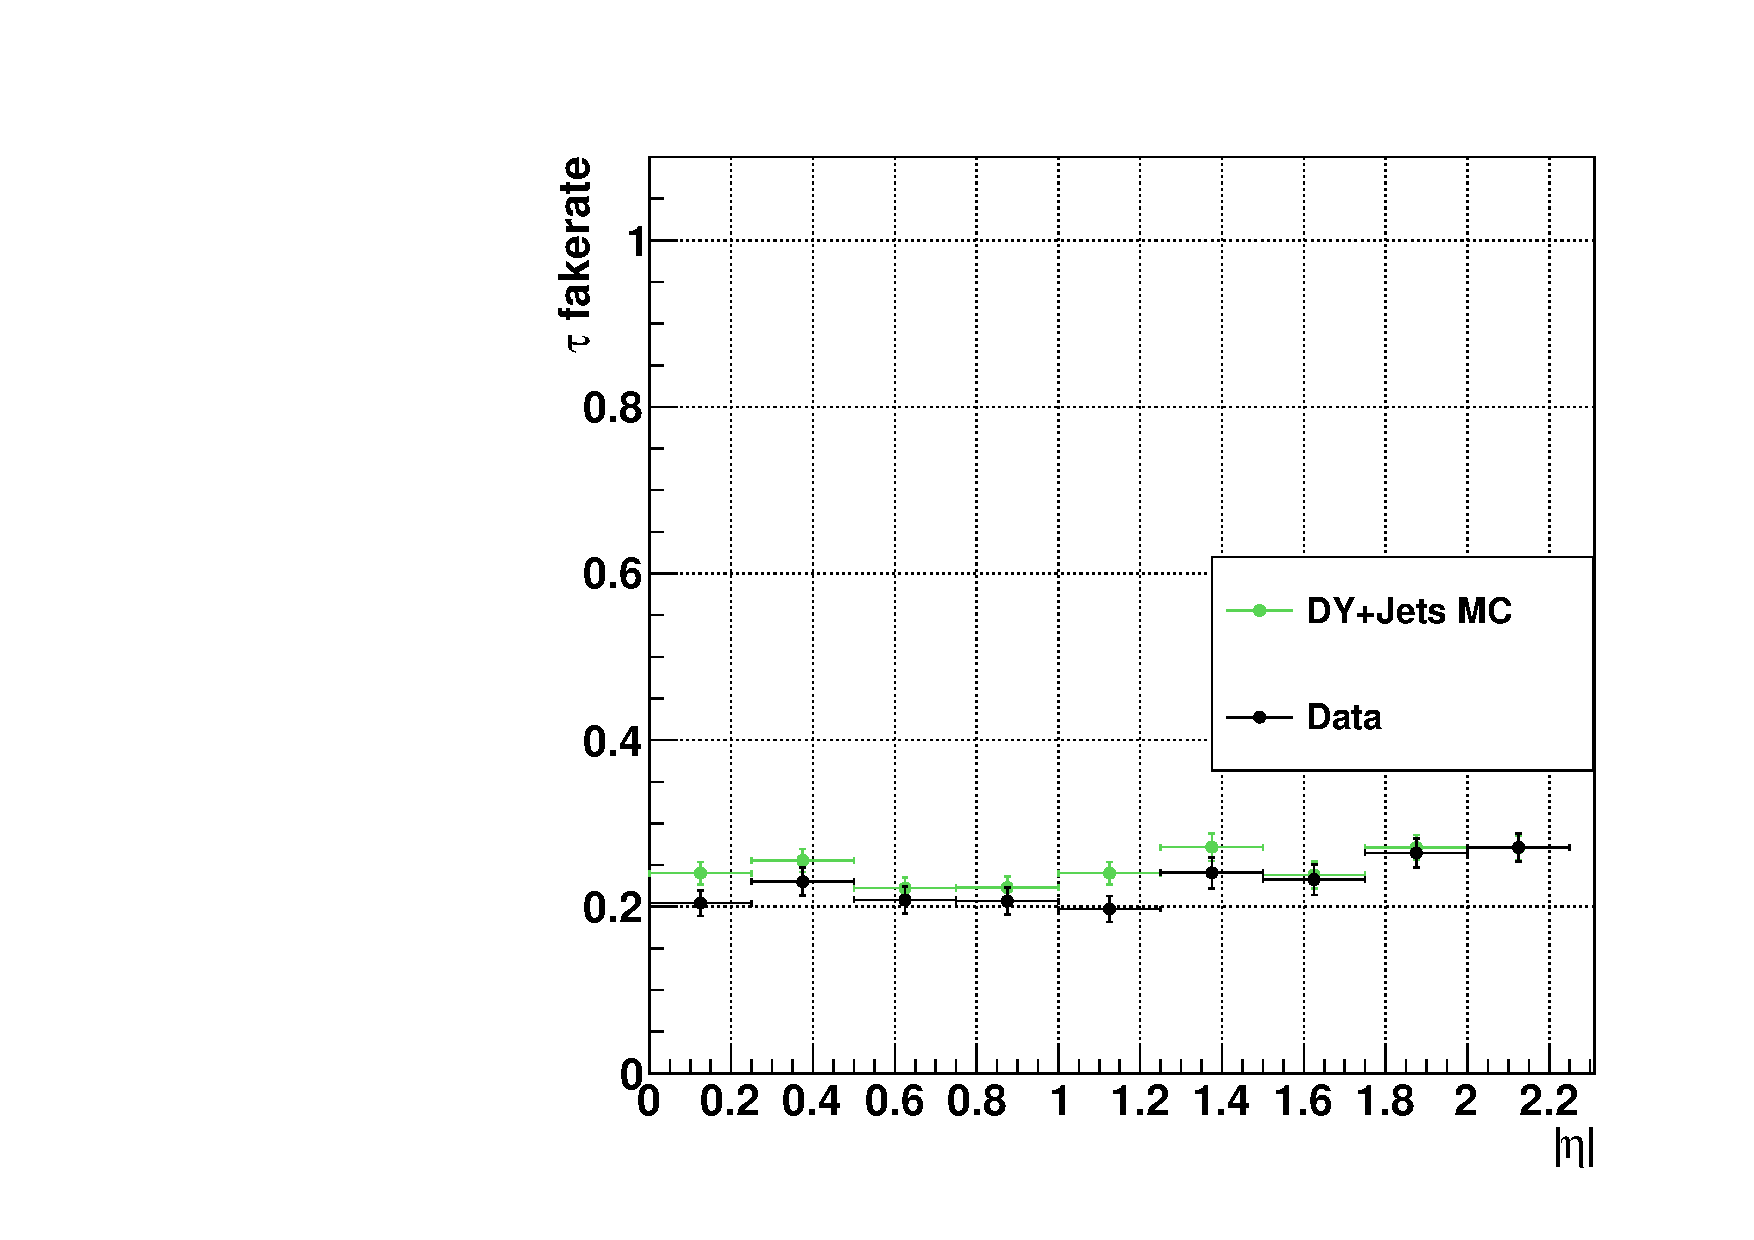
\includegraphics[width=0.3\textwidth]{chapter6/t_DM0_abstEta_fakeRate.pdf}}
        \subfigure[tau decay mode 0 vs $|\eta|$]{ 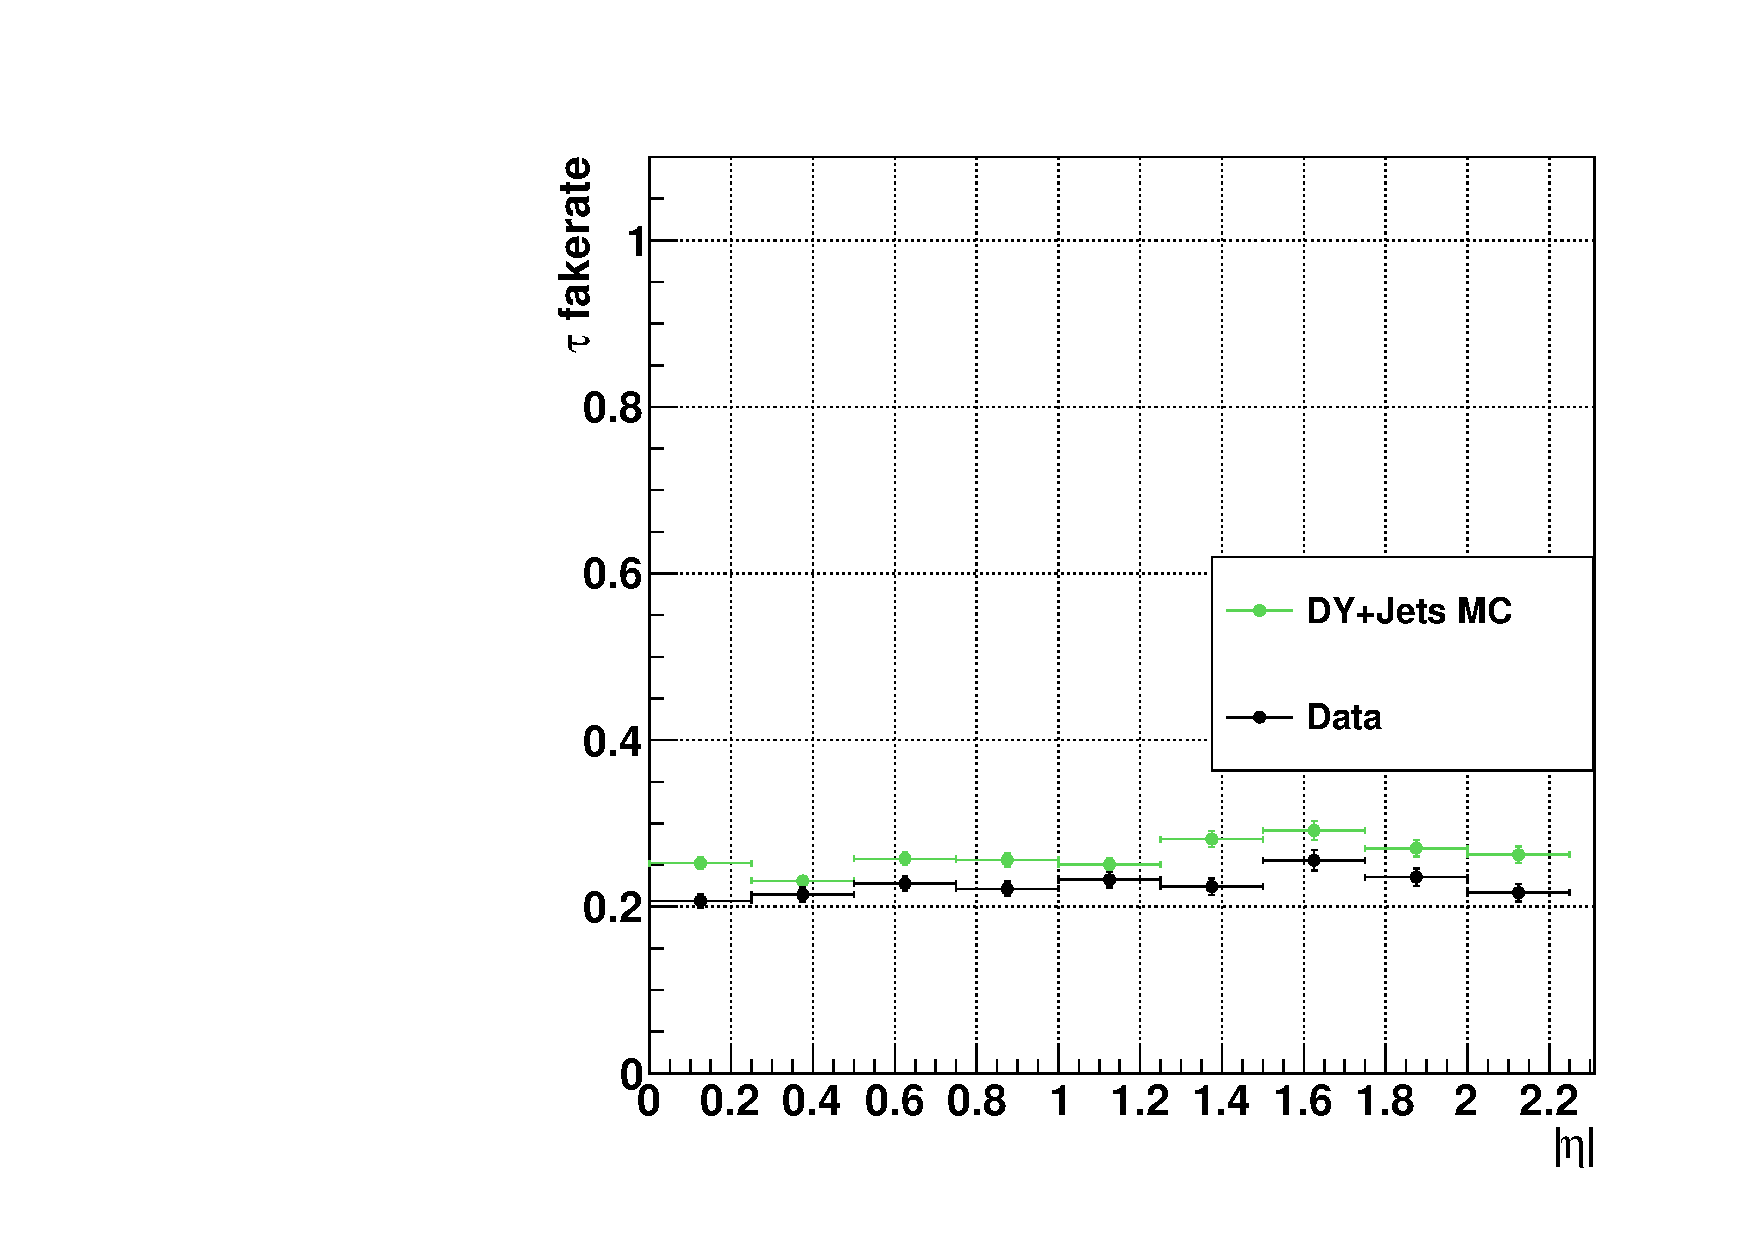
\includegraphics[width=0.3\textwidth]{chapter6/t_DM1_abstEta_fakeRate.pdf}}
         \subfigure[tau decay mode 0 vs $|\eta|$]{ 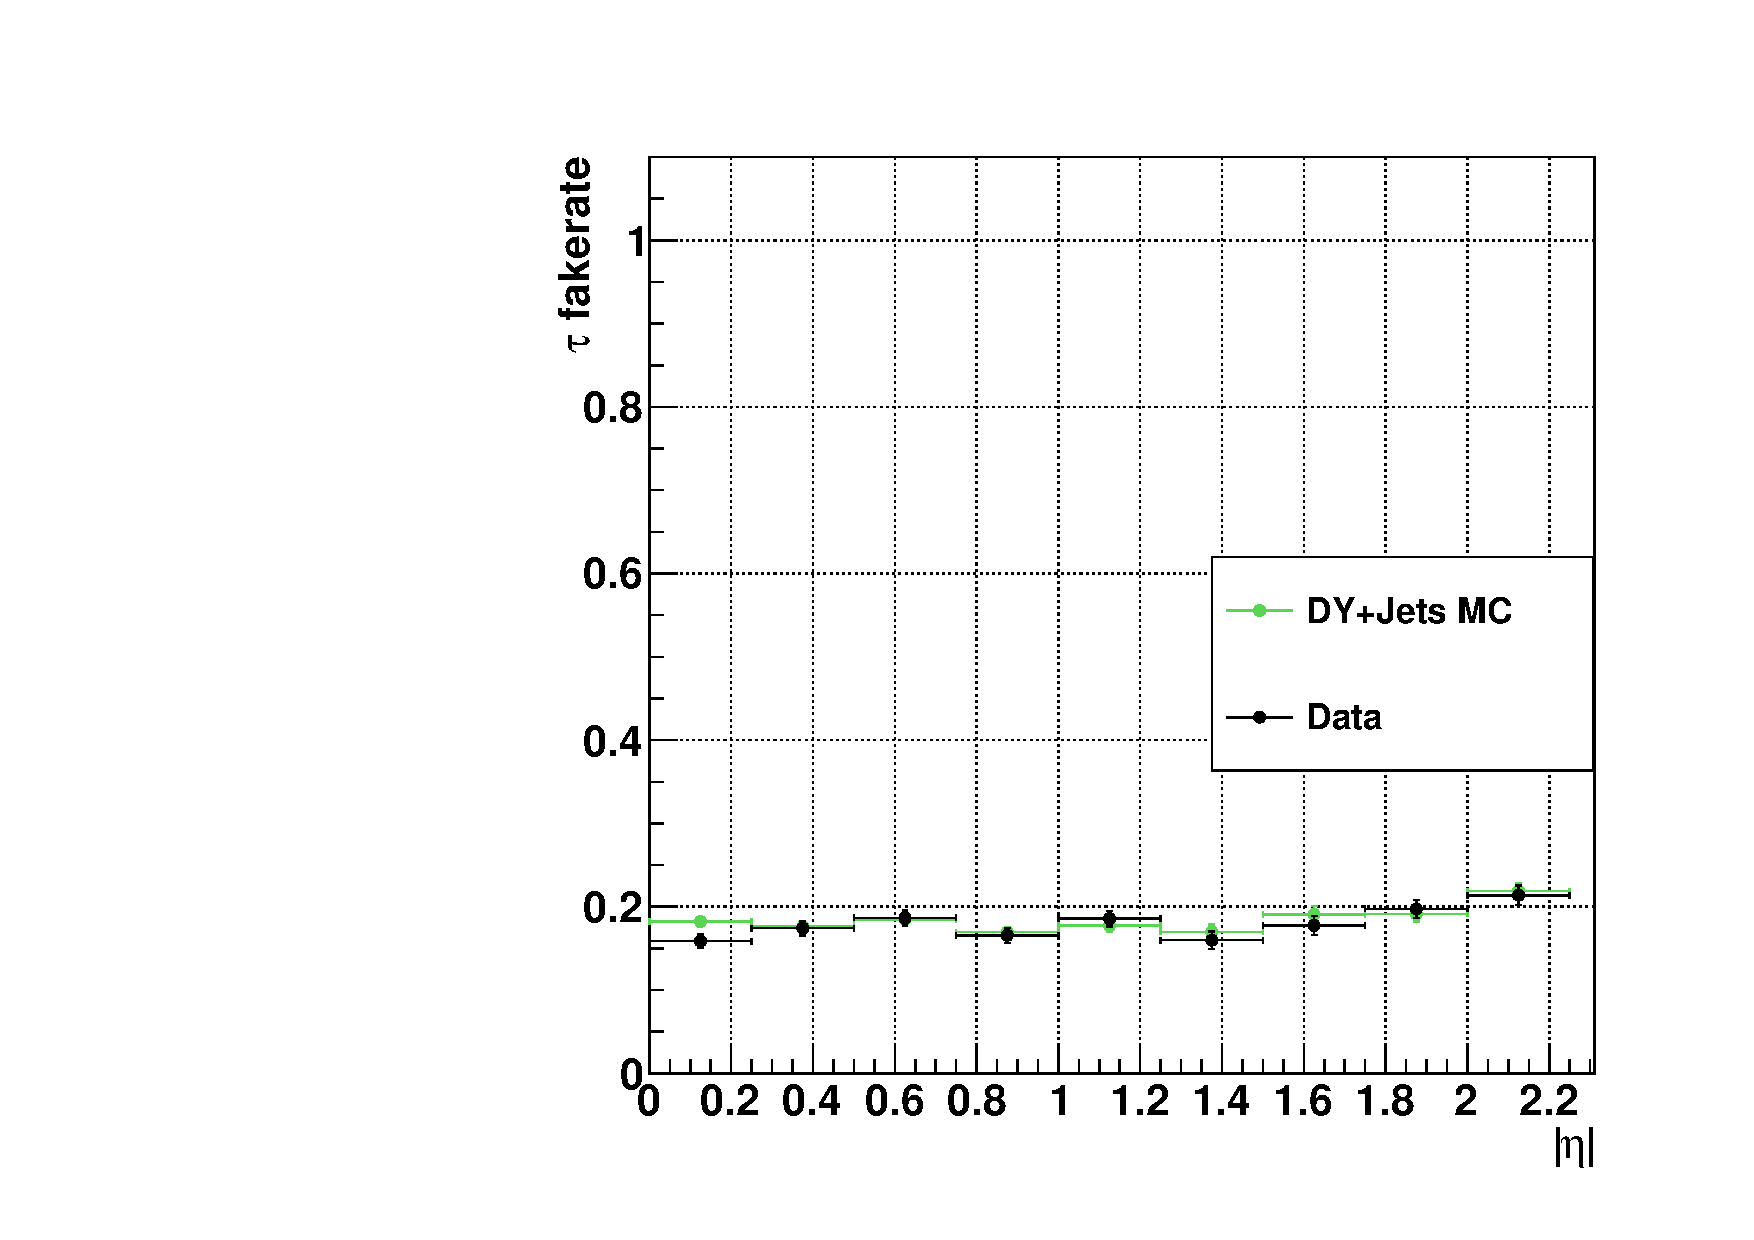
\includegraphics[width=0.3\textwidth]{chapter6/t_DM10_abstEta_fakeRate.pdf}}
     \caption{$f_{\tau}$ ratio for the $\tau$ fake rate calculation shows in term of tau decay modes, $\pt$, ECAL barrel, ECAL endcap, and $|\eta|$}
     \label{fig:fakerationumber}
\end{figure}

The estimation of $\mu$ misidentified rate the same as the $\tau$ misidentified rate, but checks if the jets in Z + jets samples pass the muon isolation. As in Equation.~\ref{eq:fakerate1}, $f_{\mu}$ is defined as the ratio between tight cut based muon isolation($I^{\mu}_{rel}<0.15$) and loose cut based muon isolation($I^{\mu}_{rel}<0.25$). The misidentified $\mu$ lepton rate $\mu(f_{\mu})$ is calculated by Equation.~\ref{eq:fakerate2}. $\mu(f_{\mu})$ is a weight to apply to Region III. In the case of estimating the misidentified $\mu$, Region III is defined as Regin I but with $\mu$ passing the loose cut based muon isolation and not passing tight cut based muon isolation. The ratio $f_{\mu}$ is shown in Figure.~\ref{fig:muonfakerationumber} in term of muon $\pt$ and $|\eta|$ distribution. 

\begin{figure}[htbp] 
     \centering
       \subfigure[$f_{\mu}$ vs $\pt$]{ 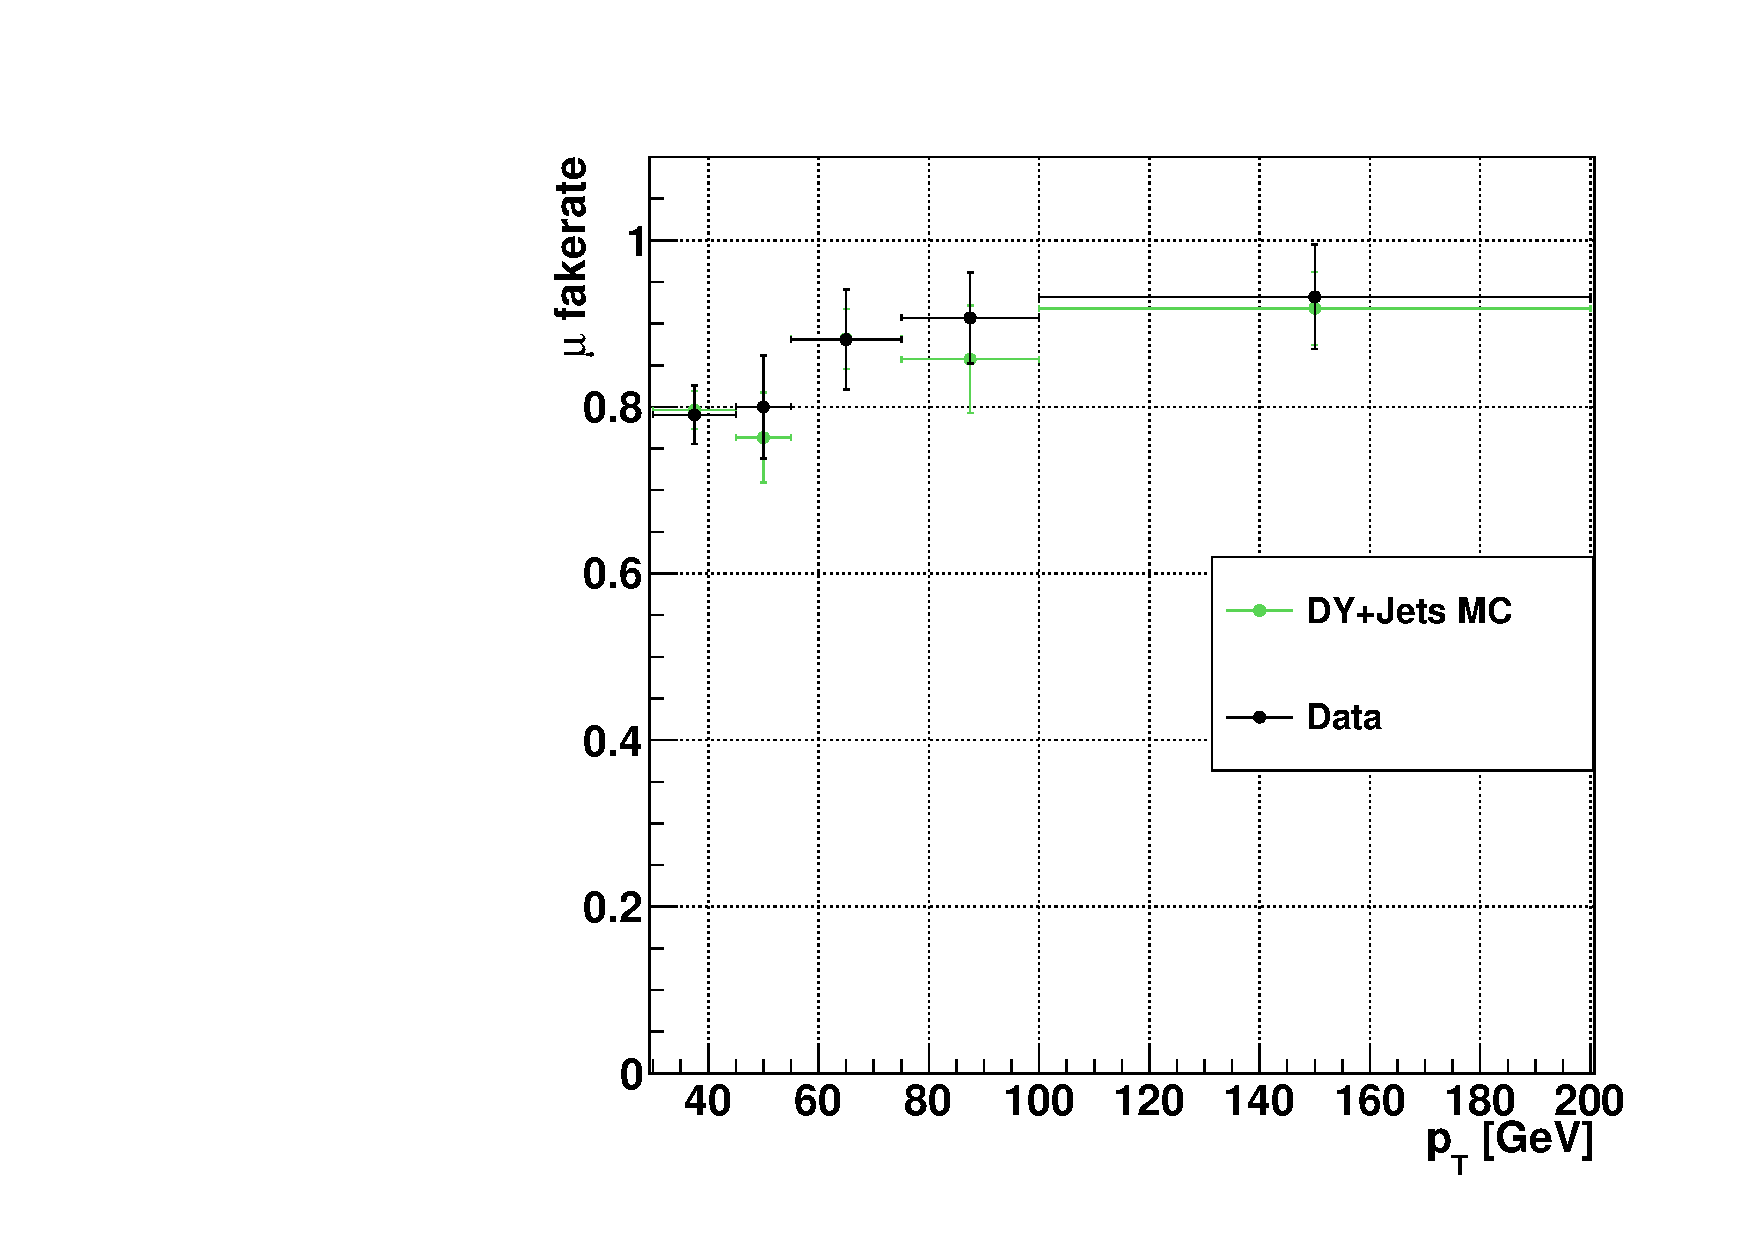
\includegraphics[width=0.3\textwidth]{chapter6/m_fakerate_0p25_pt.pdf}}
        \subfigure[$f_{\mu}$ vs $|\eta|$]{ 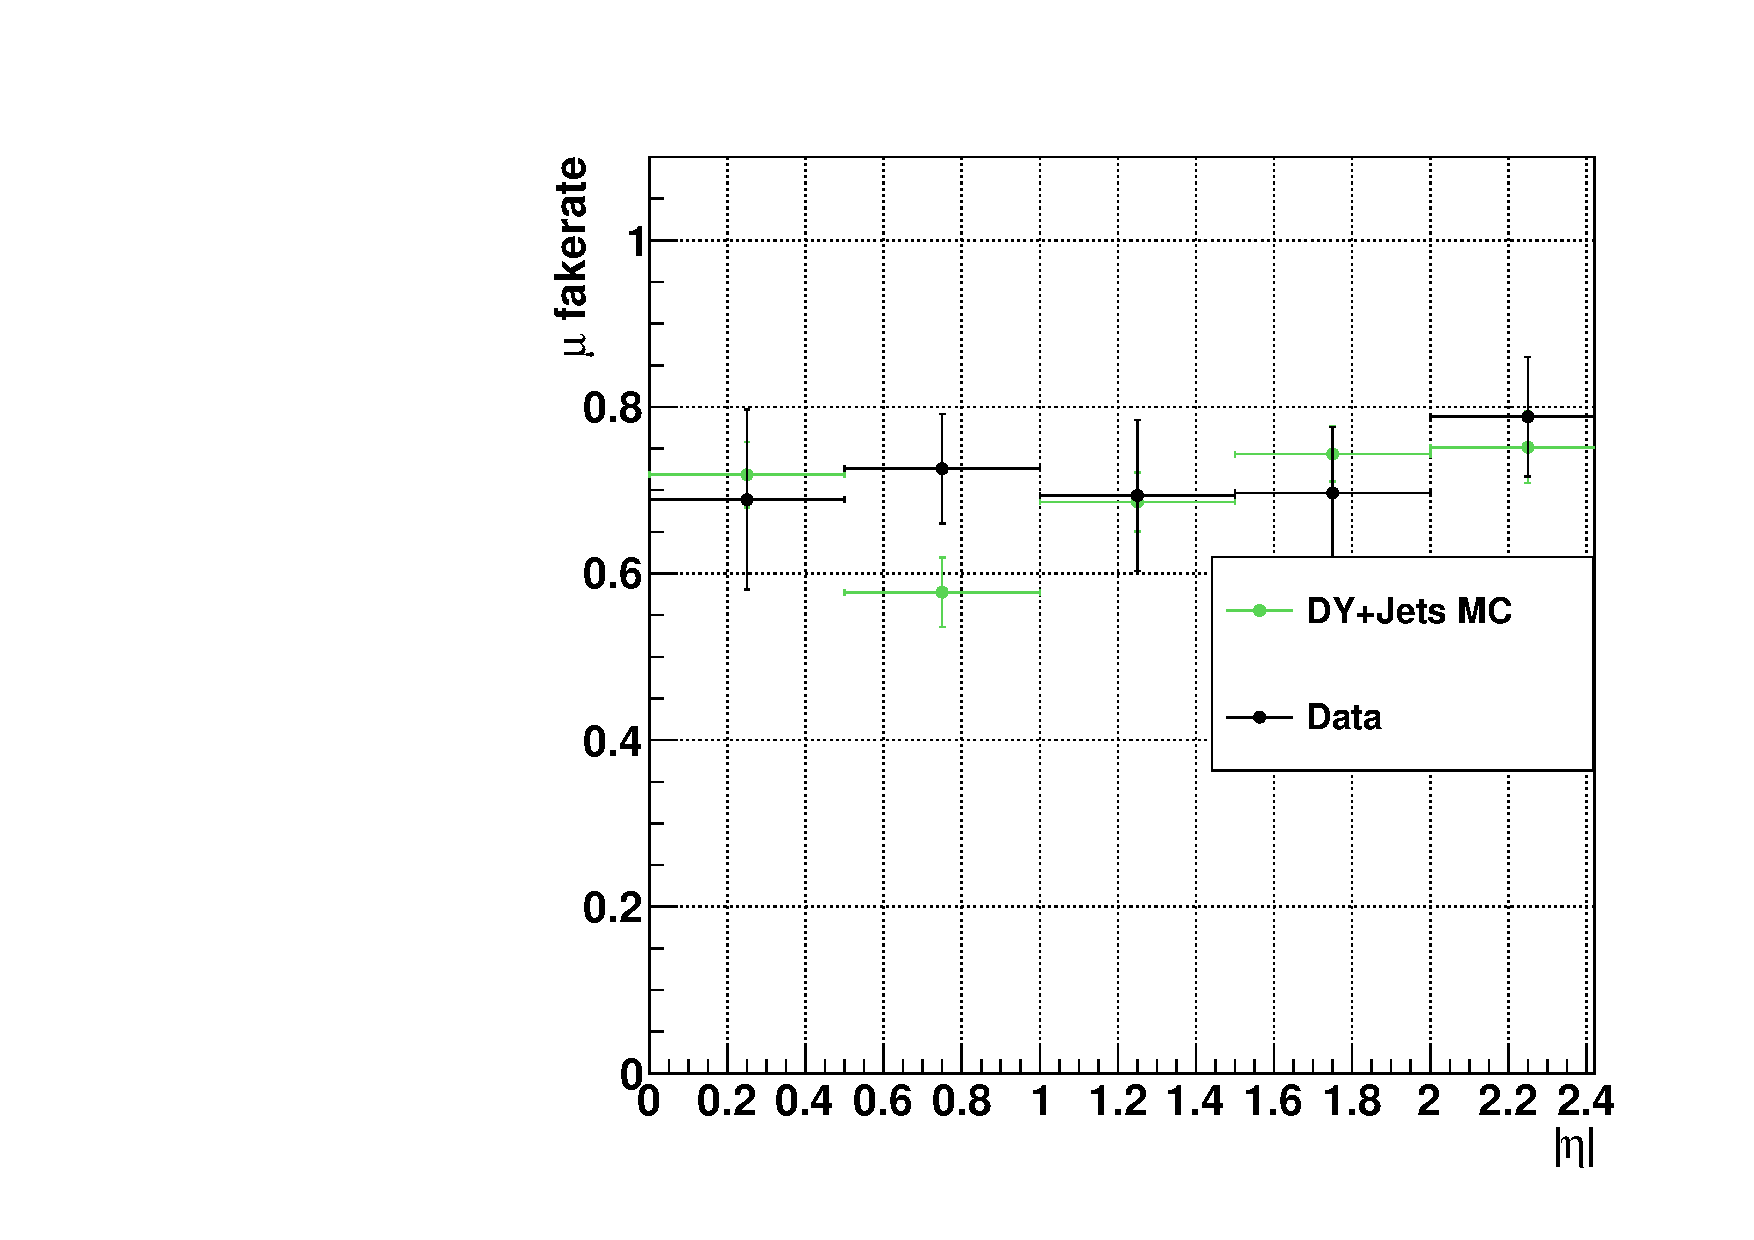
\includegraphics[width=0.3\textwidth]{chapter6/m_Loose_m3Etaabs_fakeRate}}
     \caption{$f_{\tau}$ ratio for the $\mu$ fake rate calculation shows in term of muon $\pt$ and $|\eta|$.}
     \label{fig:muonfakerationumber}
\end{figure}

There are overlap between the estimated misidentified muon and tau lepton when both of the leptons are fake ones. The overlap events are estimated as in Equation.~\ref{eq:fakerateoverlep}. In the equation, the N(Region III) stands for the events in Region III. In this case, Region III is defined as muon leptons passing the lose isolation, but not passing the tight isolation, while tau leptons pass the very loose isolation but not pass the tight isolation. The final misidentified lepton background obtained by adding the misidentified muon and tau background and deducts the overlap events between these two. 

\begin{align} 
N(\text{overlap})=\frac{f_{\tau}\cdot f_{\tau}}{(1-f_{\tau})\cdot (1-f_{\mu})}\cdot N(\text{Region\ III}) \\\label{eq:fakerateoverlep}
\end{align}



In $\Hmuhad$ channel, the validation of the misidentified lepton background with full data driven method is performed in a like-sign sample and W+jets enriched control region. The like-sign sample validation requires the events pass the loose selection, the same as the signal region, but with inverted charge. Misidentified background is enriched with the requirement of inverting charge. In the W+jets enriched control region, events that pass the loose selection are further selected with  $M_T(\tau)>60$ GeV and $M_T(\mu)>80$ GeV.  In both of the control regions, misidentified background is the dominant one, as shown in Fig.~\ref{fig:fakebackgroundValidation}. With full data driven method, applied with the $\tau(f_{\tau})$ as weight, the like-sign and W+jets control regions show good data and MC agreement. 


\begin{figure}[htbp] 
     \centering
     \subfigure[Wjets enriched control region]{ 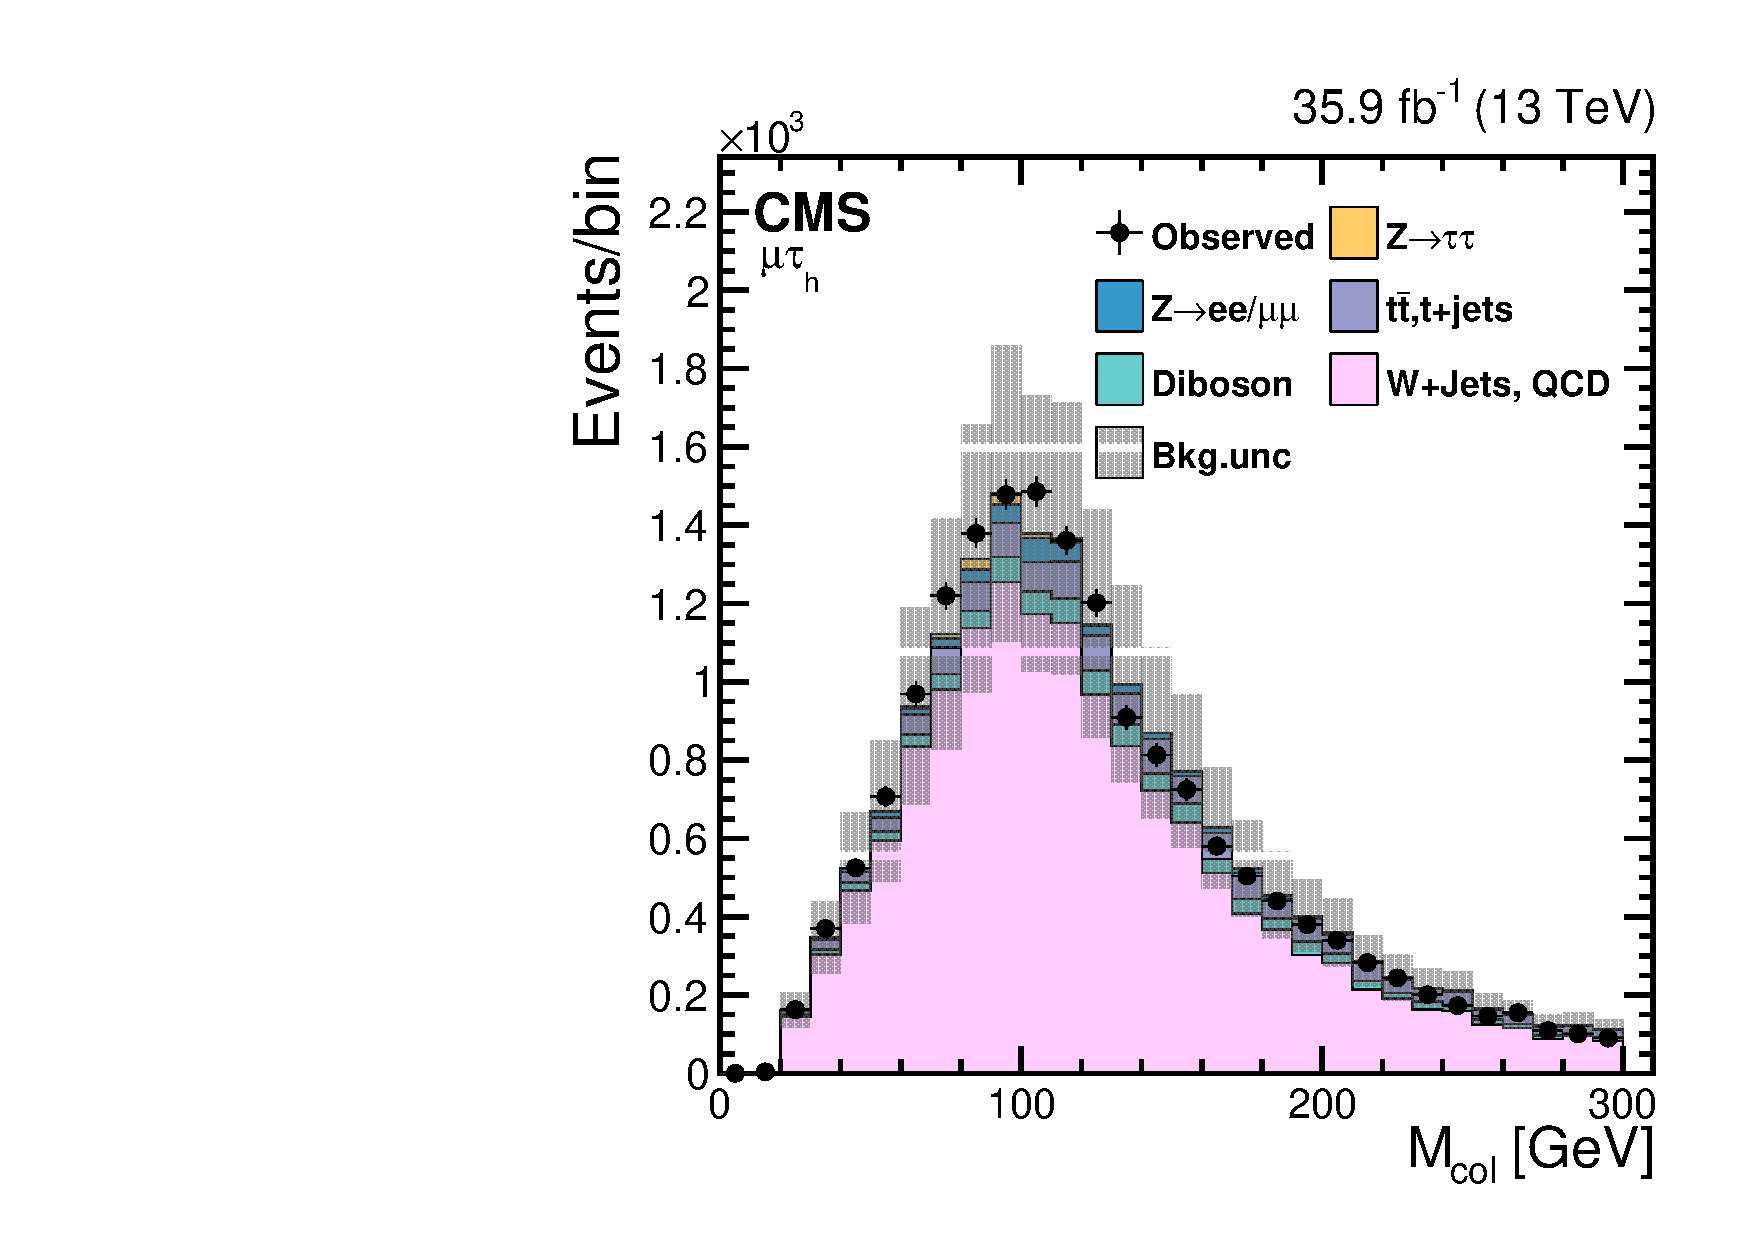
\includegraphics[width=0.4\textwidth]{chapter6/Wjets_Enriched_mutau_had01jet.pdf}}
     \subfigure[Like-sign control region]{ 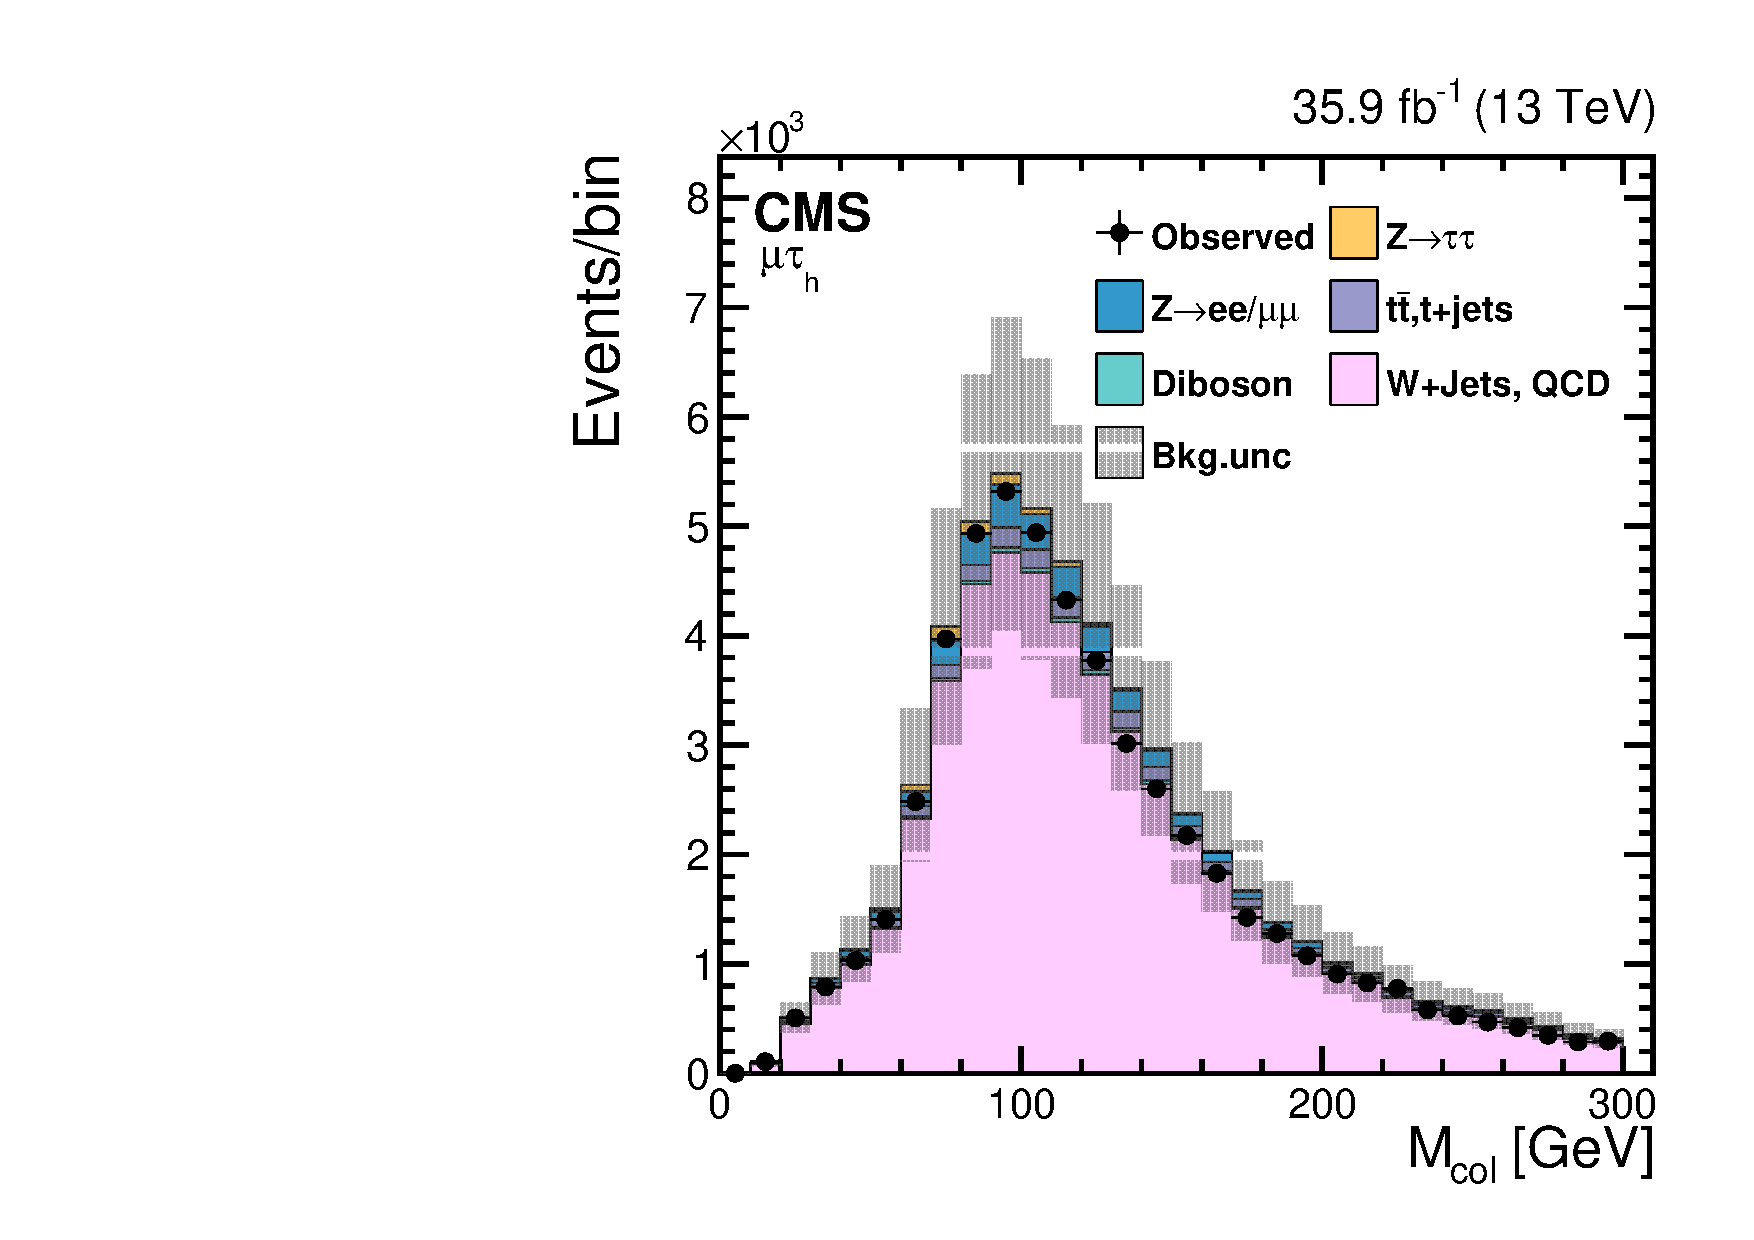
\includegraphics[width=0.4\textwidth]{chapter6/LikeSig_CR_presel_mutauh.pdf}}
     \caption{The validation of full data driven method for the misidentified lepton background. 30\% of uncertainty is assumed in both cases. }
     \label{fig:fakebackgroundValidation}
\end{figure}


\subsubsection{Other backgrounds}
Besides the misidentified background, which is composed by W+jets and QCD multi-jets background and estimated with data driven method, $Z \to \tau\tau$ and $Z \to \mu\mu$ are also major background in this analysis. In $Z \to \tau\tau$, the muons arise from a $\tau$ decay, while in $Z \to \mu\mu$, one of the $\mu$ can be misidentified as a $\tau$. In other smaller backgrounds, the $\mu\tau$ pairs can be produced from the weak decays of quarks and vector bosons. These smaller backgrounds include standard model Higgs production($H \to \tau\tau, WW$),$t\bar{t}$ ,single top quark, di-boson(WW,WZ,ZZ). A full list of background used is in the Table.~\ref{tab:mcsamples}.  These backgrounds are all estimated with MC simulation. 

In the $Z \to \mu\mu$  background, an additional scale factor is applied to the tau leptons that do not come from real taus. This is checked in the MC generator level. The scale factor is applied in term of $|\eta|$ as shown in Table.~\ref{tb:MFTcorrection}.

\begin{table}[htp]
\caption{Scale factor to the events in which a muon is misidentified as a tau}\label{tb:MFTcorrection}
\begin{center}
\begin{tabular}{|c|c|c|c|}
\hline
$|\eta|$ ranges             & Correction values \\\hline
0-0.4                             & 1.263                   \\
0.4-0.8                          & 1.364           \\
0.8-1.2                          & 0.854        \\
1.2-1.7                          & 1.712  \\
1.7-2.3                          & 2.324                                  \\\hline
 \end{tabular}
\end{center}
\end{table}







\subsection{Background estimates for $\Hehad$}

\subsubsection{Misidentified Leptons}

Misidentified lepton background is a very important one in $\Hehad$ channel. This background mainly raises from W+jets and QCD multijets. A background event passes the signal selection, may have one or both leptons are misidentified, which are faked by other objects. In $\Hehad$ 8 TeV analysis, both misidentified electron and tau leptons are considered. 

Similar to $\Hmuhad$ channel, the misidentified background in $\Hehad$ is estimated with full data driven method, with independent data sets Z+jets, in which Z bosons decay into two electrons.  Data sets are divided into four control regions for this estimation as in Table.~\ref{tab:fakeratediagram}. Region II is used to extra misidentified background in signal region, Region I, while Region II and Region IV are used for the validation of the fake rate. In the Z+jets data set selection, trigger HLT\_Ele27\_WP80 is used. The two electrons in Z+jets are required to have $\pt>30$ GeV, $|\eta|<2.3$, tight electron MVA ID and cut based tight PF isolation($I^{e}_{rel}<0.1$). The invariant mass formed by the two electrons are required to be in the Z boson mass window. Then the jets in the events are checked if they pass $\tau$ or e selection. Tau leptons should have $\pt>30$ GeV, $|\eta|<2.3$, passing tau decay mode finder and discriminator against elections and muons. Electrons pass the same conditions as the elections used in forming the Z boson mass peak, but without the requirement of isolation.  The isolation conditions are required in different conditions in the fake ratio estimation. Tau leptons use the cut based tight or loose isolation, while loose or tight MVA based electron isolation have the value $I^{e}_{rel}<0.1$ and $I^{e}_{rel}<0.2$ respectively. After the selection, the fake ratio $f_{\tau}$ is defined as the number of tau leptons passing the tight isolation divided the number of tau leptons passing the loose isolation. Similarly the fake ratio $f_{e}$ is defined as the number of elections passing the loose isolation divided by the number of electron passing the tight isolation as shown in Equation.~\ref{eq:fakerate2}. With the fake ratio $f_{\tau}$ and  $f_{e}$, the electron and tau fake rate $\tau(f_{\tau})$ and $e(f_{e})$ are estimated according to Equation.~\ref{eq:fakerate1}. The fake ratio for tau leptons and electrons are shown in Figure.~\ref{fig:fakerationumberetau}. 

\begin{figure}[htbp] 
     \centering
     \subfigure[$f_{\tau}$ vs $\pt$]{ 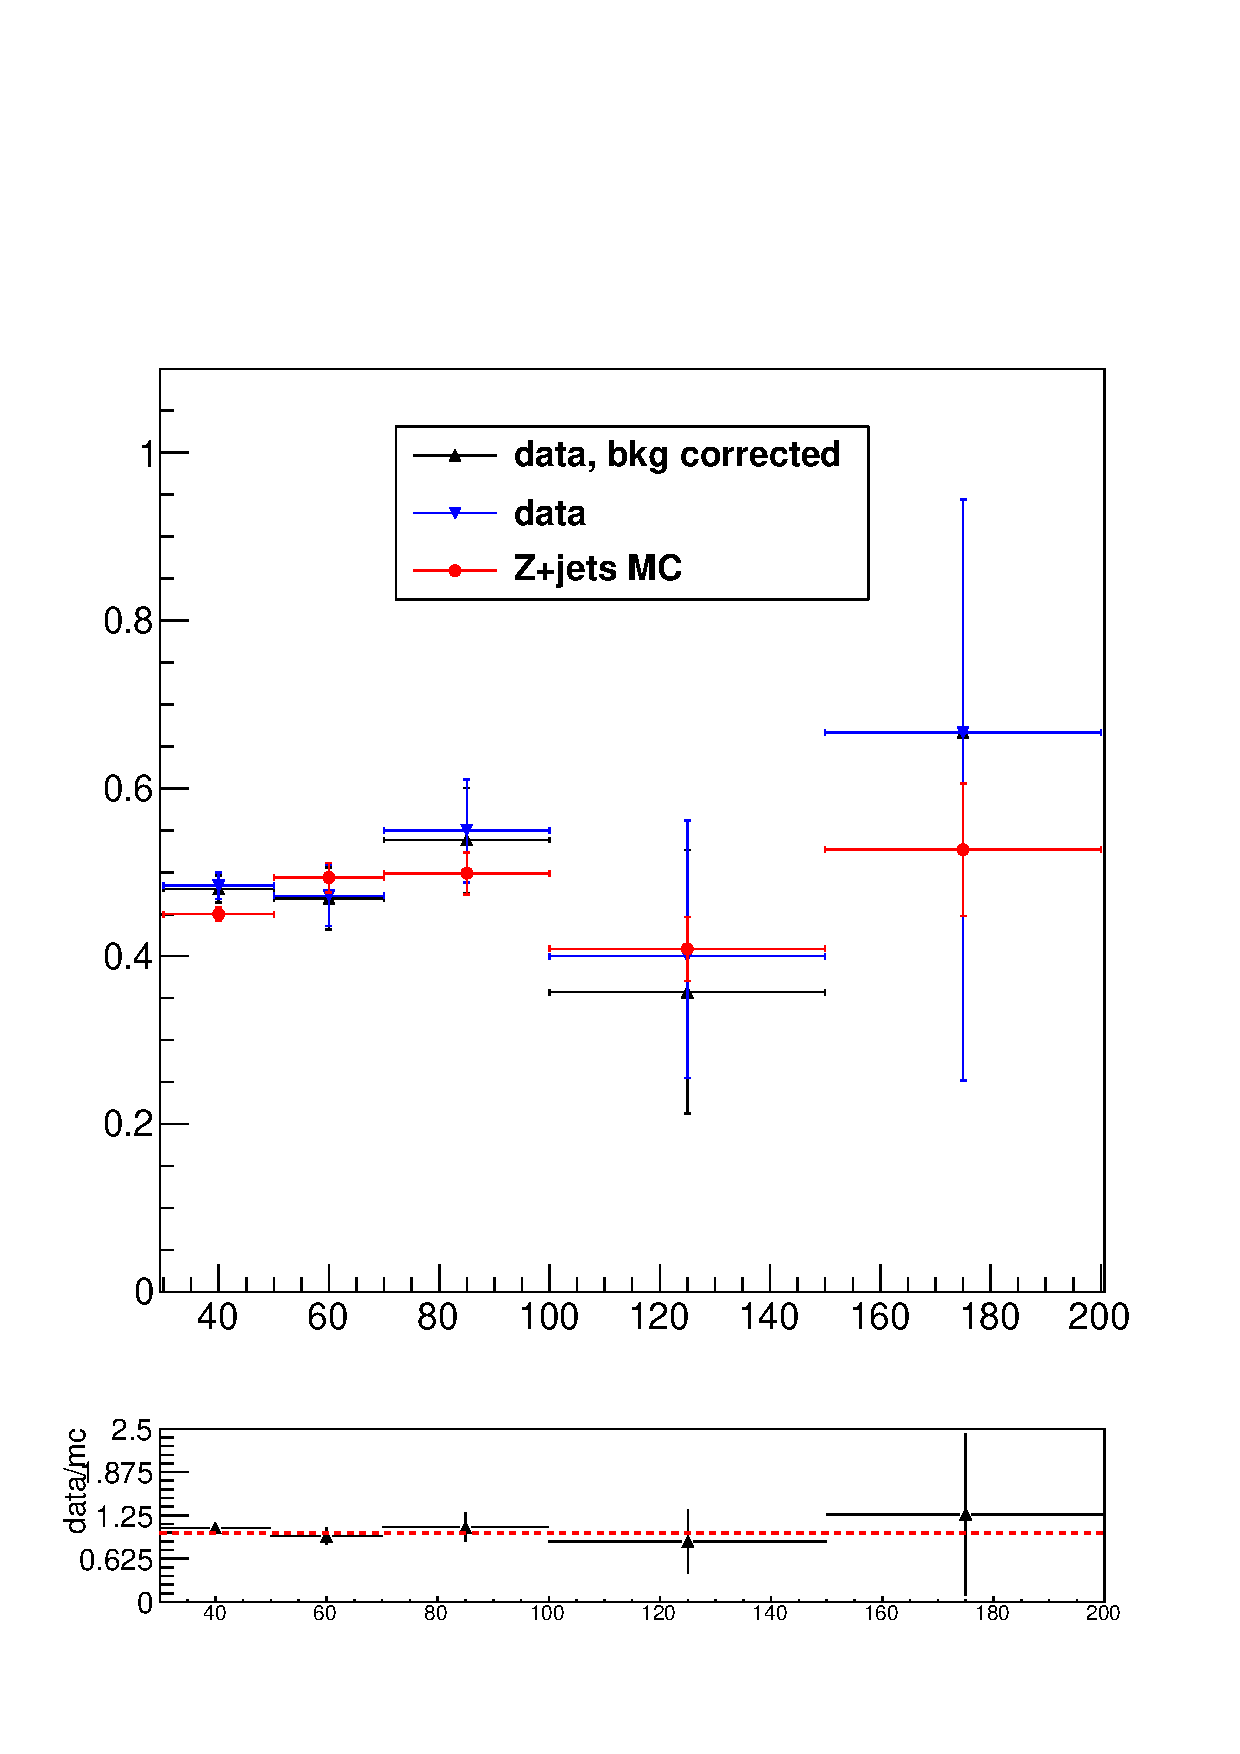
\includegraphics[width=0.4\textwidth]{chapter6/tauFakerateComparison_Pt.pdf}}
      \subfigure[$f_{\tau}$ vs $|\eta|$]{ 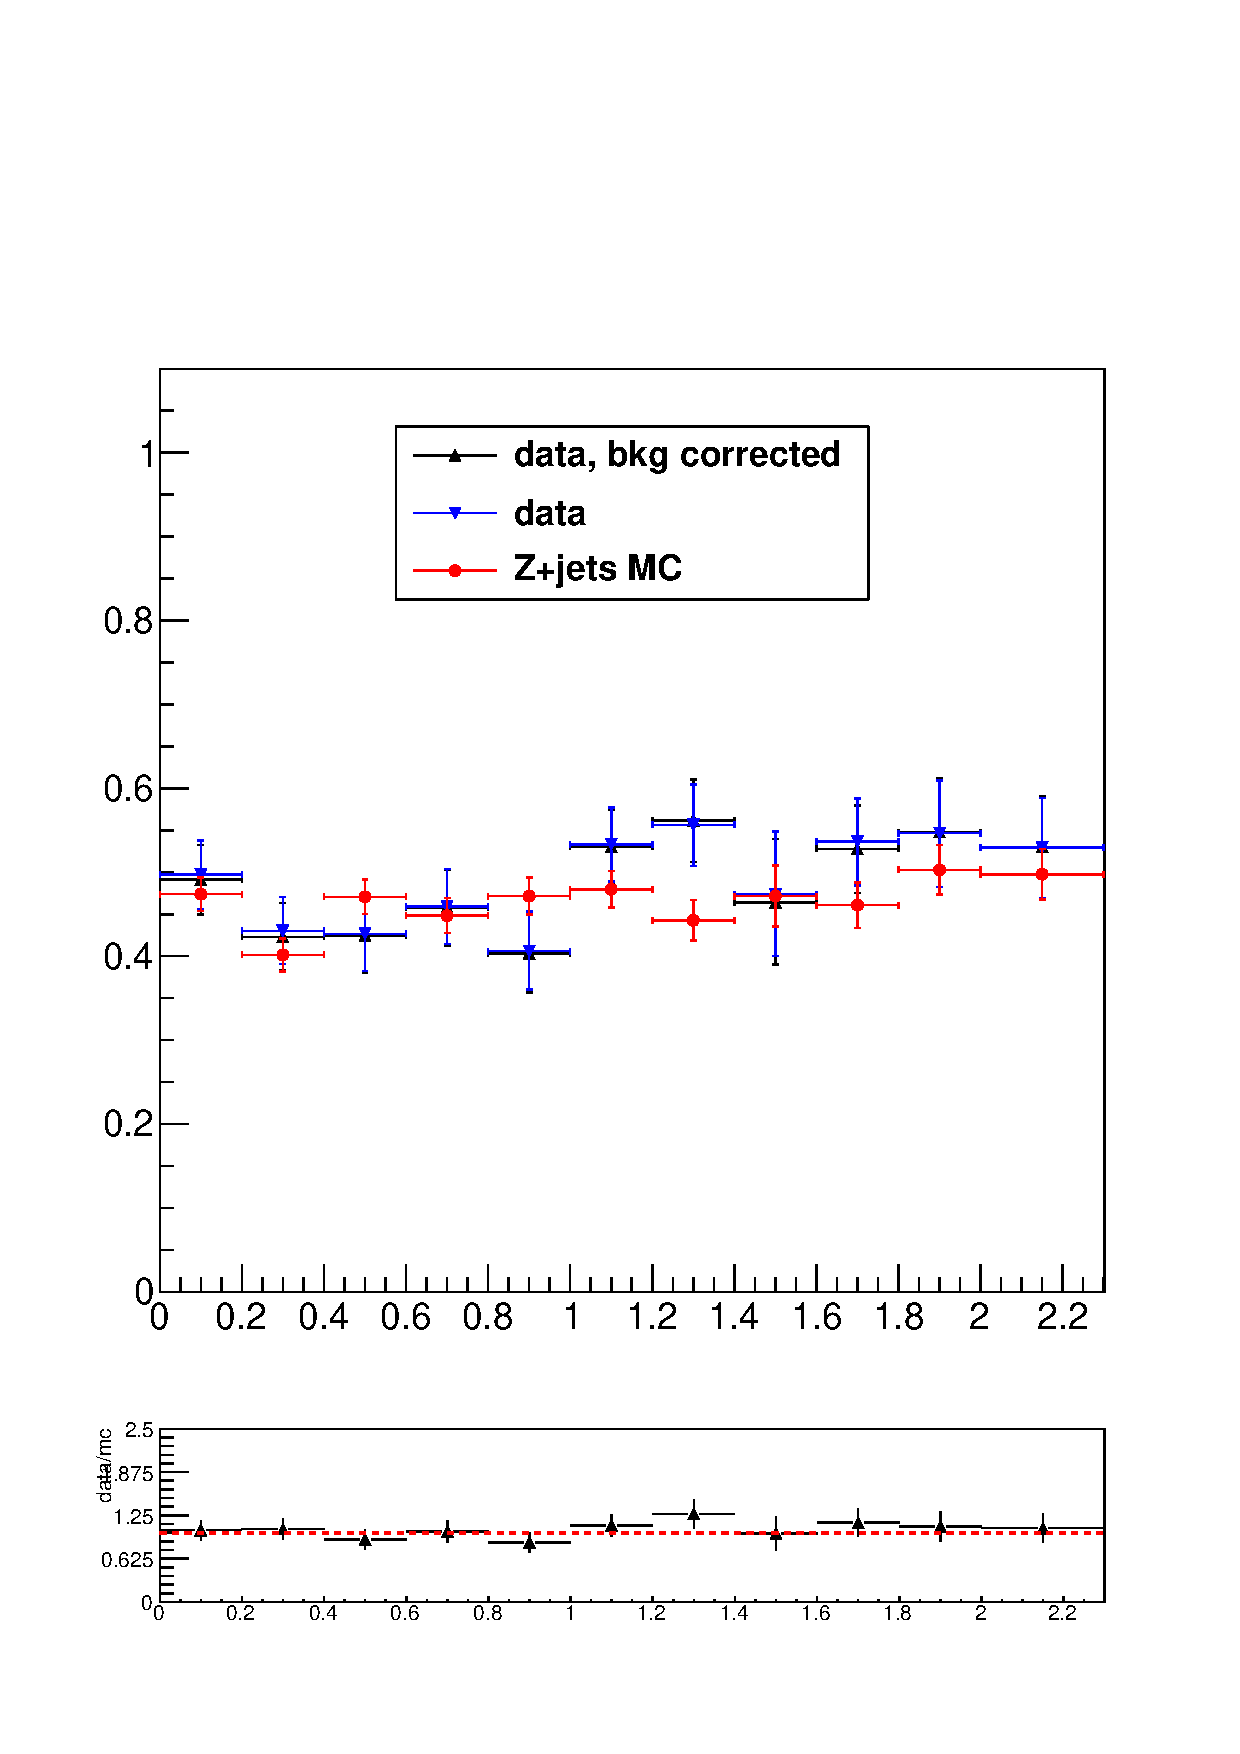
\includegraphics[width=0.4\textwidth]{chapter6/tauFakerateComparison_Eta.pdf}}
      \subfigure[$f_{e}$ vs $\pt$]{ 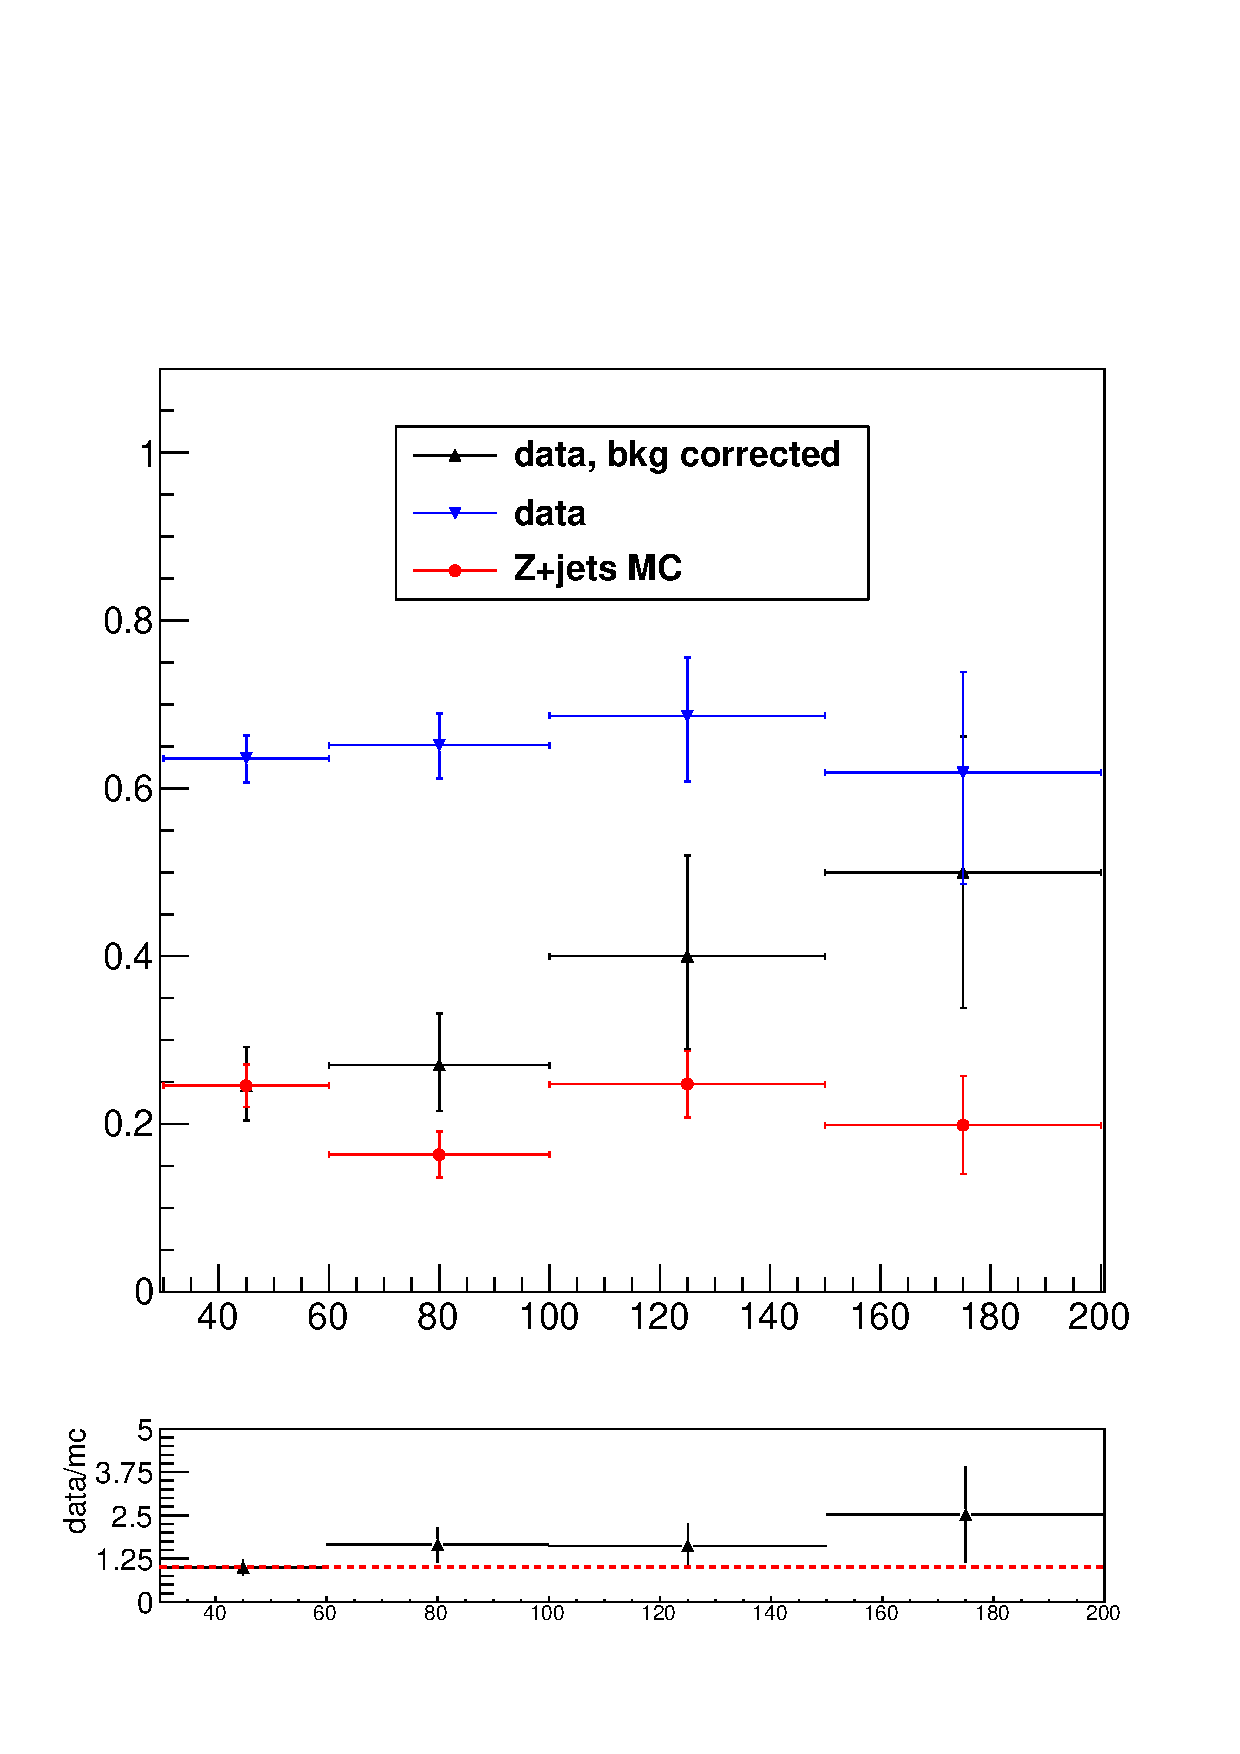
\includegraphics[width=0.4\textwidth]{chapter6/eFakerateComparison_Pt.pdf}}
     \subfigure[$f_{e}$ vs $|\eta|$]{ 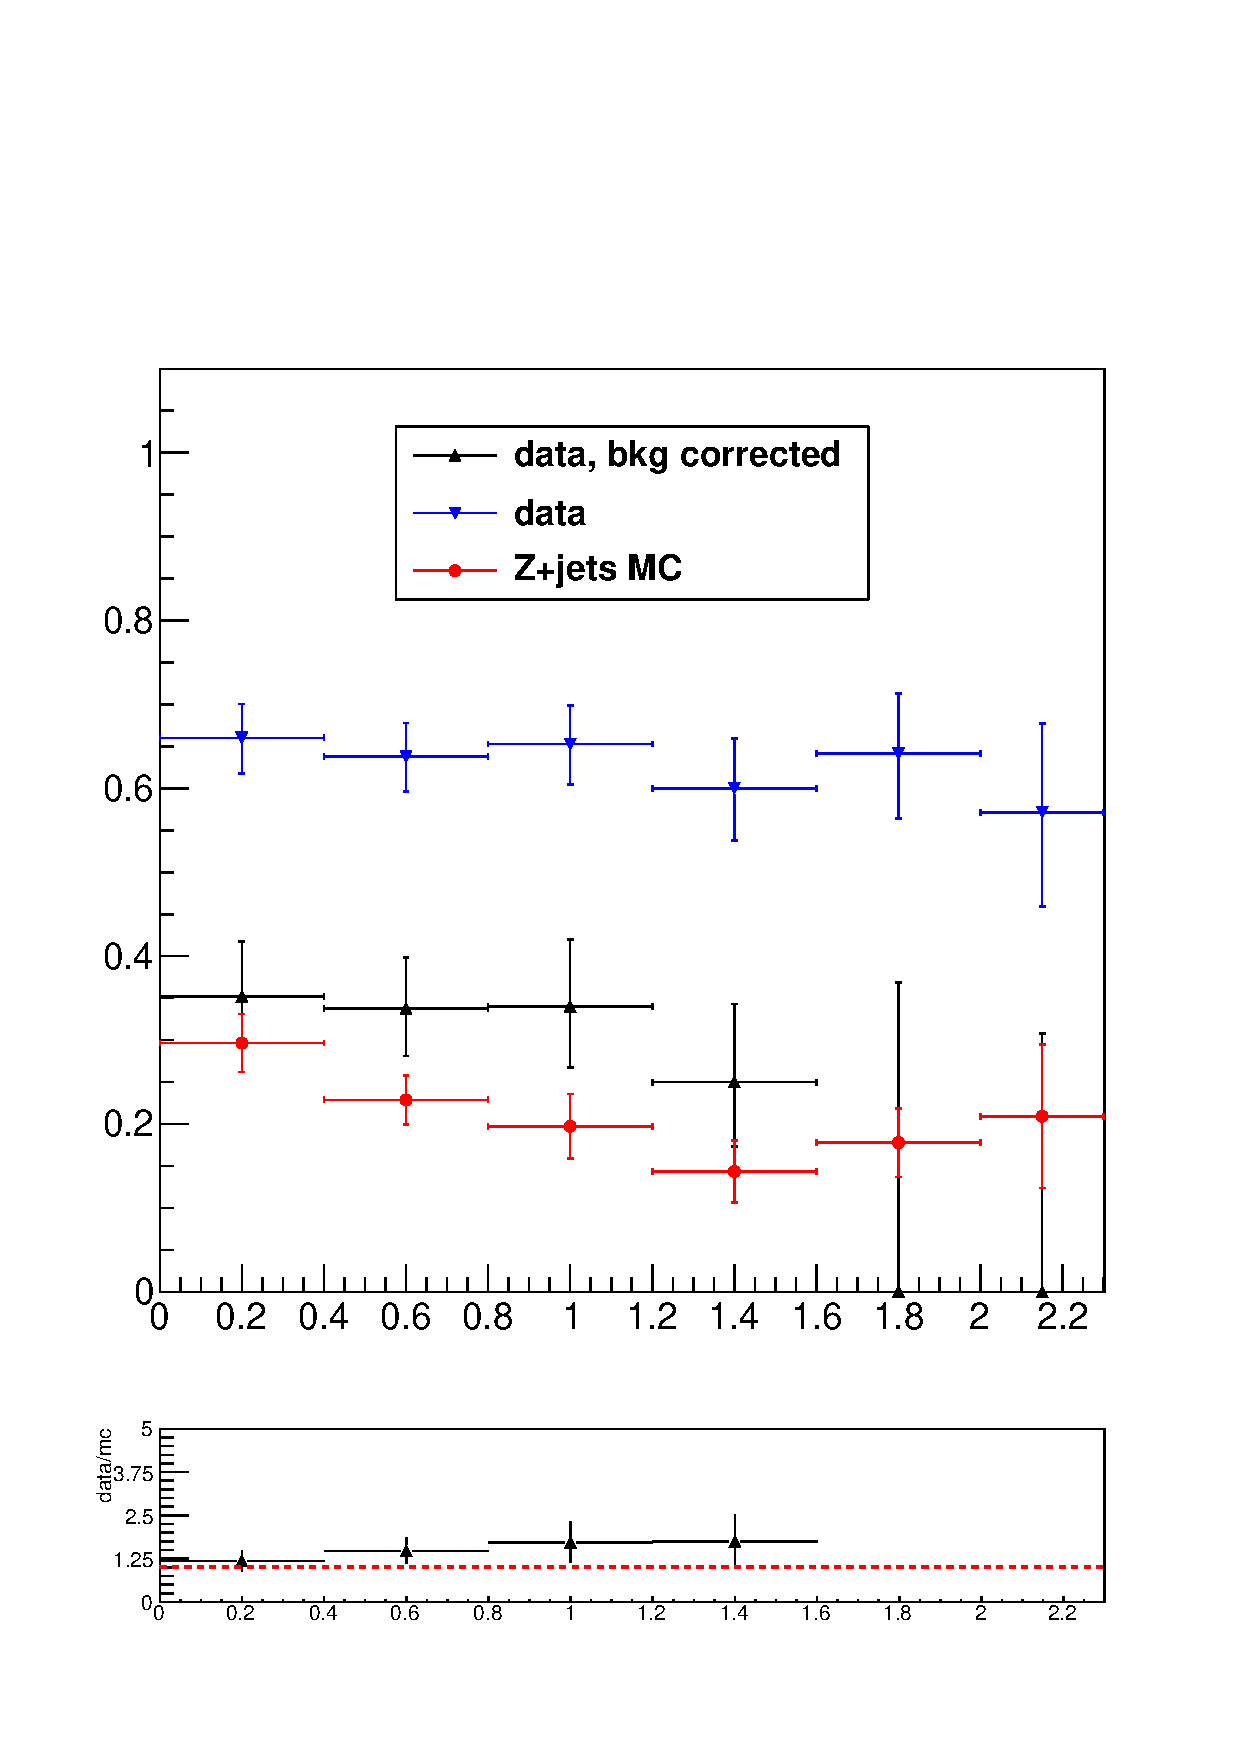
\includegraphics[width=0.4\textwidth]{chapter6/eFakerateComparison_Eta.pdf}}
     \caption{$f_{\tau}$ and  $f_{\tau}$ ratio for the fake rate calculation shows in term of  $\pt$ and $|\eta|$}
     \label{fig:fakerationumberetau}
\end{figure}


The tau and electron fake ratio is applied in term of $|\eta|$. In the estimation, the background source of three prompt leptons from Diboson samples are deducted. The tau and electron misidentified backgrounds are estimated separately, the overlap events in which both leptons are misidentified objects are estimated with Equation.~\ref{eq:fakerateoverlep}. In the equation, N(Region III) in $\Hehad$ channel satisfies the condition both leptons are loose isolated but not tight isolated.  The validation of full data driven method is done with Region II and Region IV. The distribution of the $M_{col}$ is checked in the same sign region of the two leptons, shown in Figure.~ \ref{fig:etaufakebackgroundValidationSS}, in which observed data agrees well with the events from MC and misidentified background from data driven method.


\begin{figure}[!tbp] 
\centering
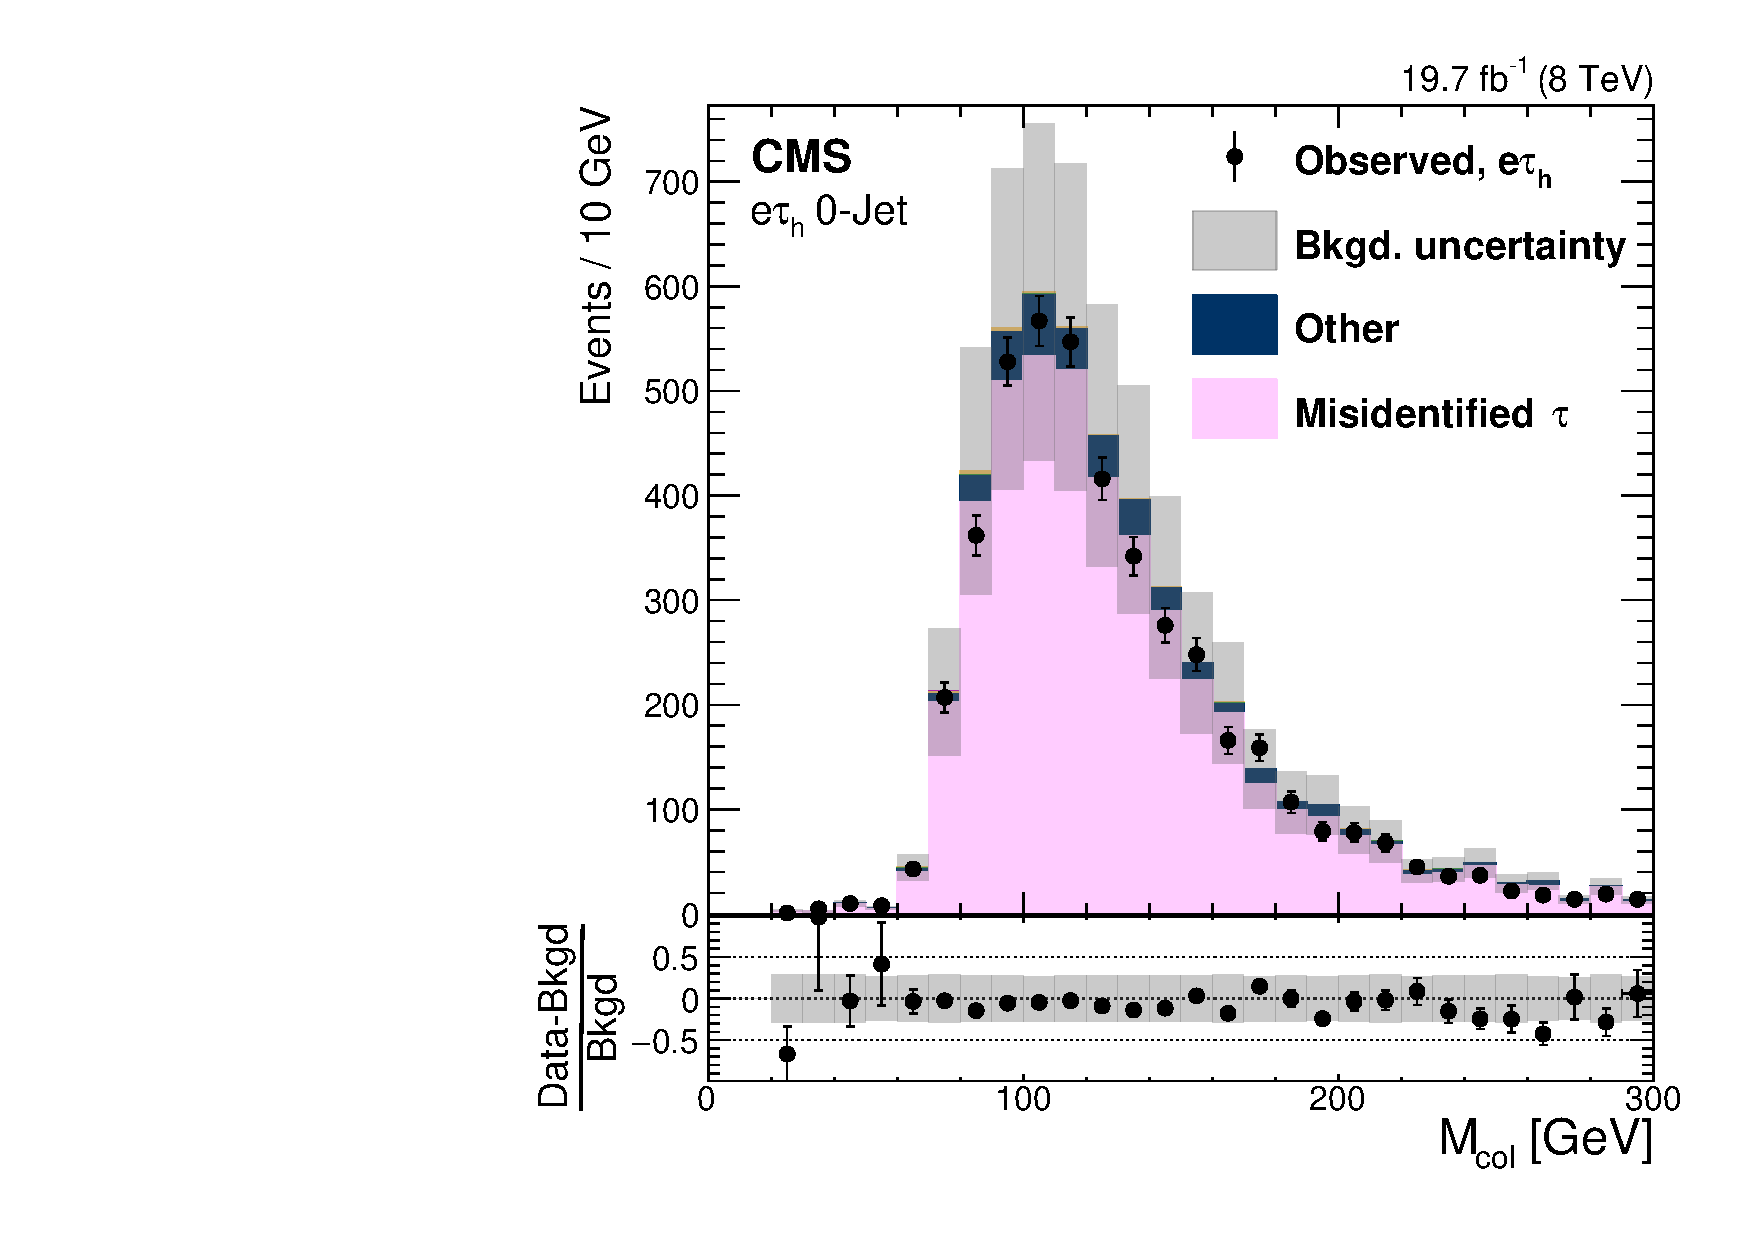
\includegraphics[width=0.4\textwidth]{chapter6/etausamesign.pdf}
\caption{Data driven method validation in Region II with e and $\tau$ leptons in same sign of charge}
\label{fig:etaufakebackgroundValidationSS}
\end{figure}

\subsubsection{$Z \to \tau \tau$}
$Z \to \tau \tau$ in another significant background in $\Hehad$ channel. In the case one of the tau leptons decay to a electron and the other hadronically decay. The background is estimated with the embedding technique\cite{Chatrchyan:2014nva}, which starts by selecting the $Z \to \mu\mu$ events from collision data. The muons pass loose muon selection and then are replaced by simulated $\tau$ leptons and reconstructed with PF algorithm. The key advantage of this technique is that the major topologies like missing energy, jet multiplicity, underlying events are directly from data. Besides tau, the other event records and detector responds are from real environment. When added to the background, the embedded data is normalized to MC prediction.  Compared with MC prediction, the visible mass peak from embedding sample shifts 2\%. This is mainly because of the difference in final-state radiation of photons between muon and tau and is corrected for. Identification and isolation correction for this shift to embedded sample are obtained by comparing with MC simulations.

\subsubsection{Other backgrounds}
$t\bar{t}$ is one of the main background. Leptonic decay W bosons can produce opposite sign lepton pair and missing energy. The shape of this background is obtained from MC samples and normalized to $t\bar{t}$ control region sample. The evens in  $t\bar{t}$ control samples are required to pass the 2-jet base selection in $\Hehad$ channel and at lease one the jets is identified as a b jet. 

The other backgrounds presented in the samples are Z+jets in which one of the electrons is misidentified as a $\tau$ lepton. Di-boson(WW,WZ,ZZ) events, single Top, SM Higgs boson production($H \to \tau \tau$)  and W$\gamma^{(\star)}$. These backgrounds are all estimated from MC simulation. 









   



